\documentclass[aps,prb,reprint,superscriptaddress,longbibliography,floatfix]{revtex4-2}
\pdftrailerid{}

\usepackage{amsmath,amssymb,bm}
\usepackage{booktabs}
\usepackage{graphicx}
\usepackage{microtype}
\usepackage{xcolor}
\usepackage{placeins}
\usepackage[colorlinks=true,citecolor=blue!55!black,linkcolor=blue!55!black,urlcolor=blue!55!black]{hyperref}

\hypersetup{
  pdftitle={Exactly Degenerate Quantum Chaos: Non-Abelian Quantum Geometry as a Probe},
  pdfauthor={Thomas J. Wang; OkongOyangO}
}

% AUTO-GENERATED FILE. DO NOT EDIT.
% Paper I empirical result macros (v13)
% registry-payload-sha256: 95c4b13c5c9ca3c42eda11fd7bef8f0bf6c2e0f86d8a7f1233cd400f1ae0e5f1
% source centered_complete_covariance_v13: ea75047473001032c1875a02944329d3db054e788945f7882d88154a7a1ee3fc
% source continuum_lll_replication_inference_v6: 21ac615ff44ddc466a1feb5c3d6f411bde9c3d34f06fb9dc570b6e77766193b6
% source cross_complete_covariance_v12: 9f5357061d9281a25483c4315da3a09c77762091e1c6754c59a8880ec16fe0e6
% source cross_mechanism_geometric_eth_v12: 18933c332747e9a134536dc06fceed5751e5575595e315e50c2f0d93e6005b86
% source lattice_susy_pilot_v10: 1a5705686a2f37f5b06216d43d8539cf15c9d6bcb92feba74e3030661d5886e8
% source matrix_element_geometric_eth_v3: bbacad6f795559f417c1e39c034a6fe51669fd509a983099c10965fb68ee34a3
% source moore_read_pilot_v9: 3024f210ca9995f57e21c9a84750a00db274b19eb63b7ee5227add45c451071e
% source spectral_silence_v2: 5a2da65d83ded56a0fbebb23f69d5c26bd41382ebaa5f32a333fb239bffd5778
% source susy_hodge_v7_N14_inference: 177643e07fc6cf210362fc1077070bd1f0ba316b6805042a626de3f96c55a627
% source topological_holonomy_v3: ff15e7cd2f947b43da5a5973bb82c50319b164877883d187c7c46b2a073823c6
% source xcube_geometric_control_v11: c75f8a27b263d71aaf1535ed0ab54f248c67335836c3543e1b95642d1ee3cc84
% source protected_scaling_inference_v4: unavailable (not tracked in delivery branch)

\newcommand{\RegisteredSourceCount}{11}
\newcommand{\SpectralKernelBandwidth}{5.7825546\times 10^{-16}}
\newcommand{\SpectralExternalGap}{0.10667223}
\newcommand{\SpectralFiberRank}{50}
\newcommand{\StoredResponseChannelConvention}{\(\widetilde X_a=-X_a\) when the source omits the Kato minus}
\newcommand{\EvenResponseContractionsSignInvariant}{\text{yes}}
\newcommand{\LaughlinDescriptiveSlopePerParticle}{-0.080934381}
\newcommand{\LaughlinNThreeRank}{16}
\newcommand{\LaughlinNThreeBasisDimension}{120}
\newcommand{\LaughlinNThreeExternalGap}{0.055871585}
\newcommand{\LaughlinNThreePhysicalTwoPairRFour}{0.37092804}
\newcommand{\LaughlinNThreeGaussianTwoPairRFour}{0.2170768}
\newcommand{\LaughlinNThreeFourthMomentExcess}{0.15385124}
\newcommand{\LaughlinNThreeStructuredTwoPairRFour}{0.31620554}
\newcommand{\LaughlinNFourRank}{25}
\newcommand{\LaughlinNFourBasisDimension}{715}
\newcommand{\LaughlinNFourExternalGap}{0.10350202}
\newcommand{\LaughlinNFourPhysicalTwoPairRFour}{0.24715444}
\newcommand{\LaughlinNFourGaussianTwoPairRFour}{0.14637654}
\newcommand{\LaughlinNFourFourthMomentExcess}{0.1007779}
\newcommand{\LaughlinNFourStructuredTwoPairRFour}{0.1829908}
\newcommand{\LaughlinNFiveRank}{36}
\newcommand{\LaughlinNFiveBasisDimension}{4368}
\newcommand{\LaughlinNFiveExternalGap}{0.093592675}
\newcommand{\LaughlinNFivePhysicalTwoPairRFour}{0.20905928}
\newcommand{\LaughlinNFiveGaussianTwoPairRFour}{0.12723201}
\newcommand{\LaughlinNFiveFourthMomentExcess}{0.081827266}
\newcommand{\LaughlinNFiveStructuredTwoPairRFour}{0.14494761}
\newcommand{\ContinuumLaughlinNThreeConnectedExcess}{0.19378584}
\newcommand{\ContinuumLaughlinNFourConnectedExcess}{0.14929835}
\newcommand{\ContinuumLaughlinNFiveConnectedExcess}{0.10502783}
\newcommand{\MooreReadNFourRank}{42}
\newcommand{\MooreReadNFourExternalGap}{1.67285}
\newcommand{\MooreReadNFourLocalTwoPairRFour}{0.50164711}
\newcommand{\MooreReadNFourStructuredTwoPairRFour}{0.58584377}
\newcommand{\MooreReadNSixRank}{120}
\newcommand{\MooreReadNSixExternalGap}{1.5351551}
\newcommand{\MooreReadNSixLocalTwoPairRFour}{0.30930182}
\newcommand{\MooreReadNSixStructuredTwoPairRFour}{0.39008828}
\newcommand{\MooreReadNFourRawMomentResidualEstimate}{0.19087579}
\newcommand{\MooreReadNFourRawMomentResidualPValue}{3.1276651\times 10^{-12}}
\newcommand{\MooreReadNFourRawMomentResidualNorm}{0.22779717}
\newcommand{\MooreReadNFourFullRFourDirectionalEstimate}{0.092095827}
\newcommand{\MooreReadNFourFullRFourLower}{-0.033378852}
\newcommand{\MooreReadNFourFullRFourPValue}{0.1136605}
\newcommand{\MooreReadNFourFullRFourZScore}{1.2072886}
\newcommand{\MooreReadNFourFullRFourCumulantNorm}{0.16101603}
\newcommand{\MooreReadNFourFullRFourFamilywiseLower}{-0.11524792}
\newcommand{\MooreReadNFourFullRFourReverseDirectionalEstimate}{0.17375367}
\newcommand{\MooreReadNFourFullRFourClaimStatus}{\text{not passed}}
\newcommand{\MooreReadNSixRawMomentResidualEstimate}{0.19360477}
\newcommand{\MooreReadNSixRawMomentResidualPValue}{3.1536978\times 10^{-15}}
\newcommand{\MooreReadNSixRawMomentResidualNorm}{0.25109352}
\newcommand{\MooreReadNSixFullRFourDirectionalEstimate}{0.18490062}
\newcommand{\MooreReadNSixFullRFourLower}{0.096705581}
\newcommand{\MooreReadNSixFullRFourPValue}{0.00028192727}
\newcommand{\MooreReadNSixFullRFourZScore}{3.4484305}
\newcommand{\MooreReadNSixFullRFourCumulantNorm}{0.21155048}
\newcommand{\MooreReadNSixFullRFourFamilywiseLower}{0.039160542}
\newcommand{\MooreReadNSixFullRFourReverseDirectionalEstimate}{0.17600677}
\newcommand{\MooreReadNSixFullRFourClaimStatus}{\text{passed}}
\newcommand{\LatticeSusyMOneRank}{2}
\newcommand{\LatticeSusyMOneExternalGap}{0.17454073}
\newcommand{\LatticeSusyMOneLocalTwoPairRFour}{0.53819492}
\newcommand{\LatticeSusyMOneIsotropicTwoPairRFour}{0.60644423}
\newcommand{\LatticeSusyMOneHodgeBalance}{0.66096261}
\newcommand{\LatticeSusyMOneRawMomentResidualEstimate}{-0.16404914}
\newcommand{\LatticeSusyMOneRawMomentResidualPValue}{0.97434241}
\newcommand{\LatticeSusyMOneRawMomentResidualNorm}{0.25622025}
\newcommand{\LatticeSusyMOneFullRFourDirectionalEstimate}{-0.15767575}
\newcommand{\LatticeSusyMOneFullRFourLower}{-0.25188284}
\newcommand{\LatticeSusyMOneFullRFourPValue}{0.99704754}
\newcommand{\LatticeSusyMOneFullRFourZScore}{-2.7530147}
\newcommand{\LatticeSusyMOneFullRFourCumulantNorm}{0.23810151}
\newcommand{\LatticeSusyMOneFullRFourFamilywiseLower}{-0.3133506}
\newcommand{\LatticeSusyMOneFullRFourReverseDirectionalEstimate}{-0.19471323}
\newcommand{\LatticeSusyMOneFullRFourClaimStatus}{\text{not passed}}
\newcommand{\LatticeSusyMTwoRank}{4}
\newcommand{\LatticeSusyMTwoExternalGap}{0.30663782}
\newcommand{\LatticeSusyMTwoLocalTwoPairRFour}{0.43553404}
\newcommand{\LatticeSusyMTwoIsotropicTwoPairRFour}{0.45406292}
\newcommand{\LatticeSusyMTwoHodgeBalance}{0.50544553}
\newcommand{\LatticeSusyMTwoRawMomentResidualEstimate}{-0.14796082}
\newcommand{\LatticeSusyMTwoRawMomentResidualPValue}{0.99937013}
\newcommand{\LatticeSusyMTwoRawMomentResidualNorm}{0.20521263}
\newcommand{\LatticeSusyMTwoFullRFourDirectionalEstimate}{-0.21481044}
\newcommand{\LatticeSusyMTwoFullRFourLower}{-0.35806588}
\newcommand{\LatticeSusyMTwoFullRFourPValue}{0.99317692}
\newcommand{\LatticeSusyMTwoFullRFourZScore}{-2.4664455}
\newcommand{\LatticeSusyMTwoFullRFourCumulantNorm}{0.25271715}
\newcommand{\LatticeSusyMTwoFullRFourFamilywiseLower}{-0.45153645}
\newcommand{\LatticeSusyMTwoFullRFourReverseDirectionalEstimate}{-0.20887386}
\newcommand{\LatticeSusyMTwoFullRFourClaimStatus}{\text{not passed}}
\newcommand{\LatticeSusyMThreeRank}{8}
\newcommand{\LatticeSusyMThreeExternalGap}{0.14619751}
\newcommand{\LatticeSusyMThreeLocalTwoPairRFour}{0.41910381}
\newcommand{\LatticeSusyMThreeIsotropicTwoPairRFour}{0.35365135}
\newcommand{\LatticeSusyMThreeHodgeBalance}{0.24583911}
\newcommand{\LatticeSusyMThreeRawMomentResidualEstimate}{0.16865522}
\newcommand{\LatticeSusyMThreeRawMomentResidualPValue}{0.070220288}
\newcommand{\LatticeSusyMThreeRawMomentResidualNorm}{0.29060309}
\newcommand{\LatticeSusyMThreeFullRFourDirectionalEstimate}{-0.035495439}
\newcommand{\LatticeSusyMThreeFullRFourLower}{-0.21443993}
\newcommand{\LatticeSusyMThreeFullRFourPValue}{0.62789119}
\newcommand{\LatticeSusyMThreeFullRFourZScore}{-0.32627325}
\newcommand{\LatticeSusyMThreeFullRFourCumulantNorm}{0.12506445}
\newcommand{\LatticeSusyMThreeFullRFourFamilywiseLower}{-0.3311967}
\newcommand{\LatticeSusyMThreeFullRFourReverseDirectionalEstimate}{-0.11551404}
\newcommand{\LatticeSusyMThreeFullRFourClaimStatus}{\text{not passed}}
\newcommand{\SusySykNFourteenMedianOne}{0.30152872}
\newcommand{\SusySykNFourteenMedianTwo}{0.37499257}
\newcommand{\XCubeCoefficientCurvature}{0}
\newcommand{\XCubeTransportCurvatureEigenvalue}{-0.5}
\newcommand{\XCubeTransportConnectedVariance}{0}
\newcommand{\HolonomyNThreeRank}{16}
\newcommand{\HolonomyNThreeChernNumber}{6}
\newcommand{\HolonomyNThreeMinimumGap}{0.051741368}
\newcommand{\HolonomyNThreeBaseGapRatio}{0.28849403}
\newcommand{\HolonomyNThreeFinalGapRatioMedian}{0.32114901}
\newcommand{\HolonomyNThreeMinimumOverlapSingularValue}{0.85325072}
\newcommand{\HolonomyNFourRank}{25}
\newcommand{\HolonomyNFourChernNumber}{10}
\newcommand{\HolonomyNFourMinimumGap}{0.094695221}
\newcommand{\HolonomyNFourBaseGapRatio}{0.30997725}
\newcommand{\HolonomyNFourFinalGapRatioMedian}{0.33175374}
\newcommand{\HolonomyNFourMinimumOverlapSingularValue}{0.83693205}
\newcommand{\RawMomentResidualRealizationCount}{24}
\newcommand{\RawMomentResidualLabelCount}{2}
\newcommand{\FullRFourTrainingCount}{12}
\newcommand{\FullRFourInferenceCount}{12}
\newcommand{\FullRFourPairingCount}{3}
\newcommand{\FullRFourFamilyAlpha}{0.05}
\newcommand{\FullRFourPerCaseAlpha}{0.01}
\newcommand{\FullRFourPrimaryFamilySize}{5}
\newcommand{\FullRFourStudentTDegreesOfFreedom}{11}


\newcommand{\Tr}{\operatorname{Tr}}
\newcommand{\cH}{\mathcal H}
\newcommand{\cQ}{\mathcal Q}
\newcommand{\cA}{\mathcal A}
\newcommand{\cK}{\mathcal K}

\begin{document}

\title{Exactly Degenerate Quantum Chaos: Non-Abelian Quantum Geometry as a Probe}

\author{Thomas J. Wang}
\email{WangTheoPhys@outlook.com}
\affiliation{Tsinghua University, Beijing 100084, China}

\author{OkongOyangO}
\affiliation{The Pennsylvania State University, University Park, Pennsylvania 16802, USA}

\date{\today}

\begin{abstract}
Exact degeneracy makes ordinary level statistics spectrally silent: within a protected rank-$D$ manifold the connected energy spectral form factor vanishes identically. It does not, however, fix how the degenerate subspace moves through Hilbert space. We formulate this motion through the non-Abelian quantum geometric tensor of the protected projector and separate protection and mixing: the traceless intrafiber response may vanish while the off-fiber response remains nonzero. We compare two- and three-body fractional-quantum-Hall parents, random and local supersymmetric cohomology, and an X-cube stabilizer control. Finite-$D$ curvature spectra show Jacobi-like local repulsion in several stochastic sectors, whereas longer-range correlations and four-point contractions retain parent- and covariance-dependent memory. For the complete fourth-order test, we subtract the exactly enumerated population mean of each registered finite ensemble, fit the channel whitener on 12 frozen panels, and evaluate 12 held-out panels with all three complex Wick pairings. With a Student-$t_{11}$ reference and a Bonferroni correction over five cases, only Moore--Read $N=6$ passes the positive directional gate; Moore--Read $N=4$ and lattice-SUSY ranks $D=2,4,8$ do not. The X-cube control has either zero curvature or deterministic scalar curvature with zero connected variance. These results establish a finite-rank, mechanism-dependent geometric distinction inside spectrally silent manifolds, not an asymptotic or universal Geometric ETH.
\end{abstract}

\maketitle

\section{Introduction}
\label{sec:introduction}

Quantum chaos is usually inferred from the spectrum.  After resolving exact
symmetries, nearby levels in a nonintegrable many-body Hamiltonian repel, and
longer-range correlations approach the appropriate random-matrix ensemble.
The same spectral viewpoint underlies much of the connection between quantum
chaos and the eigenstate thermalization hypothesis (ETH)
\cite{srednicki1994,dalessio2016}.  Wave-function chaos can also appear as
universal spectral correlations among reduced-density-matrix eigenvalues,
distinct from the energy-level point process \cite{chenludwig2018}.  The
practical starting point is nevertheless usually a nondegenerate sequence of
energies.

An exactly degenerate manifold removes that starting point.  Let a rank-$D$
subspace have energy $E_0$ and remain separated from its complement by a
positive gap.  Within this subspace every level spacing is zero.  Unfolding is
undefined, the spacing ratio is trivial, and the contribution of the manifold
to the spectral form factor is silent about how its states mix: it depends on
$D$ and $E_0$, not on the orientation of the subspace in the ambient Hilbert
space.  This spectral silence does not classify the Hamiltonian as integrable
or chaotic.  Exact equality of energies can follow from symmetry multiplets, a
common kernel of positive constraints, supercharge cohomology, or dependent
commuting stabilizers.  Each mechanism can coexist with a large and highly
structured complement.

The missing information is carried by the motion of the spectral projector.
For a smooth family $H(\boldsymbol\lambda)$, denote the protected projector by
$P(\boldsymbol\lambda)$ and its complement by $Q=1-P$.  Kato's formulation of
adiabatic transport makes $P$, rather than a basis chosen inside its range,
the natural object \cite{kato1950}.  The Abelian geometric phase
\cite{berry1984}, its non-Abelian extension for degenerate multiplets
\cite{wilczekzee1984}, and the quantum metric
\cite{provostvallee1980} all arise from derivatives of this projector.  The
rectangular operator
\[
 X_a=Q(\partial_aP)P
\]
is the off-fiber projector response: it records how a coupling displacement
rotates protected states into the positive-energy complement.  Products
$X_a^\dagger X_b$ form the non-Abelian quantum geometric tensor, and their
antisymmetric part gives a curvature acting within the protected fiber.
Unlike raw Berry-connection entries, its spectrum and traced contractions are
gauge invariant.

Geometry has already proved sensitive to chaos in nondegenerate many-body
eigenstates \cite{pandey2020}.  More directly relevant here, non-Abelian
Berry curvature was proposed as a chaos probe for exactly degenerate BPS
microstates, where conventional level statistics cannot resolve dynamics
inside the protected sector \cite{chen2026}.  We ask the corresponding
condensed-matter question: what statistical structure can the projector
response retain when degeneracy is enforced algebraically, rather than
obtained by tuning unresolved levels together?  The aim is not to replace
spectral chaos by a single geometric number.  It is to determine which
features of random-matrix behavior survive in the geometry, which remain
sensitive to the parent Hamiltonian, and which exact mechanisms force a
structured negative control.

Two distinctions are essential.  The first separates protection from mixing.
For $h_a=\partial_aH$, the traceless intrafiber perturbation
\[
 S_a=Ph_aP-\frac{\Tr(Ph_aP)}{D}P
\]
tests first-order splitting, whereas $X_a$ tests motion of the subspace.
Along an exactness-preserving transport, $S_a=0$ and the rank and external gap
remain fixed, yet $X_a$ can be nonzero.  Degeneracy and geometric mixing are
therefore independent response channels.  This observation also prevents a
common false inference: a frustration-free or supersymmetric parent need not
have trivial geometry merely because its protected energy is pinned exactly.

The second distinction concerns how a tangent is realized.  An
exactness-preserving transport is a finite family of constraints or generators
for which the common kernel stays exactly degenerate.  In the clustered Hall
parents studied below, differentiating an invertible transport of the constraint
map gives $S_a=0$ identically.  By contrast, the Laughlin fixed-parent
base-point probes apply local potentials at a single exact parent.  They
define the linear response of an isolated rank-$D$ cluster, but a generic
finite displacement splits that cluster.  We keep these two constructions
separate: holonomy and finite-path statements use only the first, while the
second supports only base-point response statistics.

Once the spectrum is silent, the statistical question also divides into
scales.  At the local level we compare curvature eigenvalues with the
finite-rank complex Jacobi process associated with products and compressions
of random subspaces \cite{collins2005}.  Jacobi-like local eigenvalue
repulsion is evidence for correlated mixing within one curvature matrix; it
does not imply that all response entries are independent Gaussian variables.
At the matrix level the two-point covariance and pseudocovariance retain the
tangent labels, complement indices, fiber indices, and parent Hamiltonian.
At fourth order one must subtract all three complex Wick contractions using
that complete covariance.  We refer to the surviving dependence of global
statistics on this tensor structure as global covariance memory.  Local
random-matrix-like repulsion and global covariance memory are compatible, and
their coexistence is one of the central finite-size observations tested here.

Our comparison is organized by the origin of exact degeneracy.  Two-body
Laughlin zero modes are realized in the Kapit--Mueller Chern band and in an
independent continuum lowest-Landau-level construction.  Three-body
Moore--Read zero modes change the clustering constraint and greatly enlarge
the protected rank.  A random cubic supercharge and a local lattice
$\mathcal N=2$ supercharge realize two inequivalent cohomological kernels.
The periodic X-cube stabilizer code supplies an exactly soluble structured
control.  Topological stability under gapped local deformations motivates the
use of projector transport in the Hall setting \cite{hastingswen2005}, but
topology alone does not determine the local curvature statistics.  The models
therefore vary the protection algebra, the locality of the tangent, and the
accessible response channels rather than serving as interchangeable
realizations of one ensemble.

The corrected fourth-order comparison is narrower than the model list. After exact population centering for each registered finite ensemble, channel whitening on a frozen 12-panel training split, and complete three-pairing Wick subtraction on 12 held-out panels, only the registered finite-rank Moore--Read $N=6$ case passes the positive directional gate under a Student-$t_{11}$ reference with a Bonferroni correction over five primary cases. Moore--Read $N=4$ and the lattice-SUSY ranks $D=2,4,8$ do not pass. No corresponding centered full-cumulant statement is assigned to the Laughlin or random-SYK production data. This pattern establishes neither Gaussian closure in the nonpassing cases nor a common ensemble across mechanisms; it fixes the claim boundary of the global comparison.

The resulting claim is deliberately finite.  We find finite-rank,
cross-mechanism evidence that exact spectral degeneracy can coexist with an
informative and, in several stochastic sectors, locally Jacobi-like quantum
geometry.  The response nevertheless remembers its constraint algebra and
operator class through its covariance and branch structure.  The X-cube
control makes the distinction sharp: coefficient deformations have zero
projector curvature, while a chosen unitary transport has deterministic
curvature whose connected variance vanishes.  Thus exact degeneracy alone
does not produce geometric chaos.

These calculations do not constitute an asymptotic Geometric ETH theorem. They neither establish a common scaling limit nor identify a single model/operator class that can be held fixed across all mechanisms. The complete-covariance inference is accepted only for the registered Moore--Read $N=6$ cell whose statistical-unit and familywise gates pass; nonpassing and untested cells are not promoted to conclusions. Section~\ref{sec:protected-response} develops the protected response formalism, Sec.~\ref{sec:statistics} fixes the hierarchy of statistics and inference units, and Sec.~\ref{sec:models} defines the exact mechanisms and tangent classes. The remaining sections present the mechanism-resolved calculations, the topological comparison, and the limits of the geometric interpretation.


\begin{figure*}[t]
  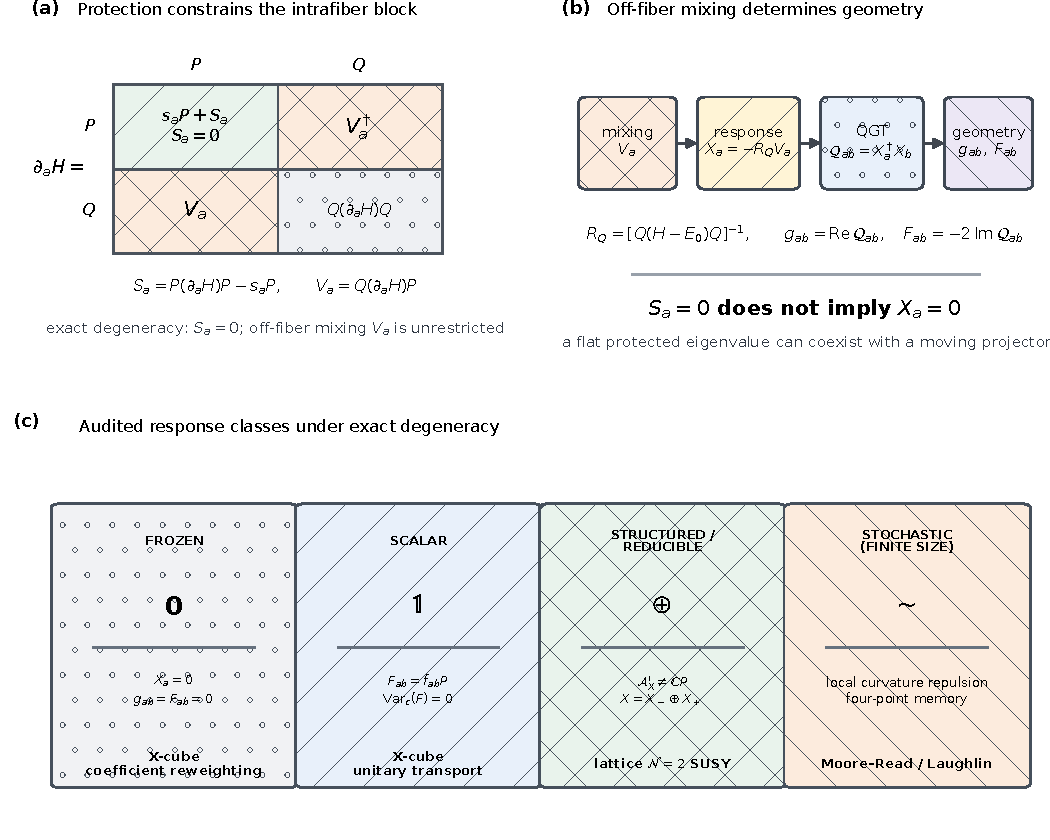
\includegraphics[width=\textwidth]{figures/figure_1_protection_mixing_v13.pdf}
  \caption{\label{fig:protection}Protection and mixing channels under exact degeneracy. (a) The tangent $\partial_aH$ is decomposed with respect to the protected projector $P$ and its complement $Q$. Exact first-order protection constrains the traceless intrafiber block $S_a=P(\partial_aH)P-s_aP$, where $s_a=D^{-1}\Tr[P(\partial_aH)P]$, but leaves the off-fiber mixing $V_a=Q(\partial_aH)P$ unrestricted. (b) The reduced resolvent converts this mixing into the Kato response $X_a=-R_QV_a$, from which $\mathcal Q_{ab}=X_a^\dagger X_b$, $g_{ab}$, and $F_{ab}$ follow; hence $S_a=0$ does not imply $X_a=0$. (c) The audited responses divide into frozen, scalar, structured/reducible, and stochastic finite-size classes. X-cube coefficient reweighting and unitary transport realize the first two classes, the local lattice-$\mathcal N=2$ supercharge resolves into exact/coexact branches, and the clustered Hall parents provide the stochastic examples. The classification concerns projector response and does not assign level statistics or thermalization to the protected manifold.}
\end{figure*}

\section{Protected fibers and off-fiber response}
\label{sec:protected-response}

Let $H(\boldsymbol\lambda)$ be a differentiable family of self-adjoint
Hamiltonians.  Throughout this paper, $E_0(\boldsymbol\lambda)$ denotes an
isolated eigenvalue of constant multiplicity $D$ on the parameter region under
consideration, and $P(\boldsymbol\lambda)$ is its constant rank $D$ spectral
projector.  We write
$Q=1-P$ and assume a nonzero spectral gap
$\Delta=\operatorname{dist}[E_0,\operatorname{spec}(QHQ)]$.  These assumptions
are stronger than observing a numerically narrow band: they ensure that the
projector is differentiable and that the inverse of $H-E_0$ on $Q\cH$ is
bounded.  No response formula below is continued through a point at which the
rank changes or the spectral gap closes.

\subsection{The splitting and mixing blocks}

For a coordinate $\lambda^a$, set $h_a=\partial_aH$.  The two blocks of $h_a$
that are relevant to the protected fiber are
\begin{equation}
 S_a=Ph_aP-\frac{\Tr(Ph_aP)}{D}P,
 \qquad
 V_a=Qh_aP .
 \label{eq:splitting}
\end{equation}
The Hermitian operator $S_a$ is the traceless intrafiber splitting channel,
whereas $V_a$ maps the protected fiber into its orthogonal complement.  If the
eigenvalue remains exactly $D$-fold degenerate along the path, differentiating
$HP=E_0P$ and projecting with $P$ on both sides gives
$Ph_aP=(\partial_aE_0)P$, hence $S_a=0$.  This is a local necessary condition
for an exactness-preserving path.  It is not, by itself, a claim that an
arbitrary linear perturbation with $S_a=0$ preserves the degeneracy at finite
amplitude; the finite path must continue to satisfy the rank and gap
conditions.

Crucially, $S_a=0$ imposes no corresponding condition on $V_a$.  Exact
degeneracy fixes the restriction of the Hamiltonian to $P\cH$, but it does not
fix how that subspace is embedded in the full Hilbert space.  This distinction
also works in the opposite direction.  An intervention supported entirely in
$P\cH$ can make $S_a$ nonzero, and can even produce random-matrix level
statistics inside the multiplet, while keeping the projector fixed.  Such an
intervention changes intrafiber energies but produces no quantum geometry.

\subsection{Reduced response of an isolated fiber}

Under the assumptions above, the reduced resolvent
\[
 R_Q=Q\bigl[Q(H-E_0)Q\bigr]^{-1}Q
\]
exists and satisfies $\lVert R_Q\rVert\leq\Delta^{-1}$.  Projecting the
derivative of $HP=E_0P$ from $P\cH$ to $Q\cH$ gives the off-fiber response
\begin{equation}
 X_a=Q(\partial_aP)P=-R_QV_a .
 \label{eq:response}
\end{equation}
Thus a large response can arise either from a large coupling matrix element
$V_a$ or from a small excitation denominator.  The distinction matters when
systems with different gaps are compared: an unnormalized response does not,
by itself, measure more effective mixing channels.  Equation~\eqref{eq:response}
also makes the domain of the calculation explicit.  It is an adiabatic
response of an isolated spectral subspace, not a prescription for following a
collection of levels after that subspace touches the rest of the spectrum.

The matrix-valued quantum geometric tensor is the operator on $P\cH$
\begin{equation}
 \mathcal Q_{ab}
 =P(\partial_aP)Q(\partial_bP)P
 =X_a^\dagger X_b,
 \qquad
 g_{ab}=\frac{\mathcal Q_{ab}+\mathcal Q_{ba}}{2}.
 \label{eq:qgt}
\end{equation}
The diagonal $g_{aa}=X_a^\dagger X_a$ is positive semidefinite, and its rank
counts the fiber directions resolved by tangent $a$, subject to the gap
weighting in $R_Q$.  Unlike the scalar quantum metric of a nondegenerate
state, the off-diagonal $g_{ab}$ is generally a matrix inside the protected
multiplet; no analogous rank interpretation is assigned to it.

Choose a local orthonormal frame $\Psi=(|u_1\rangle,\ldots,|u_D\rangle)$ for
$P\cH$.  With the canonical convention
$A_a=i\Psi^\dagger\partial_a\Psi$, the non-Abelian Berry curvature is
\begin{equation}
 \begin{split}
 F_{ab}&=\partial_aA_b-\partial_bA_a-i[A_a,A_b]\\
 &=i(\mathcal Q_{ab}-\mathcal Q_{ba})
 =i\,P[\partial_aP,\partial_bP]P .
 \end{split}
 \label{eq:curvature}
\end{equation}
For $D=1$, this convention reduces to
$F_{ab}=-2\operatorname{Im}\mathcal Q_{ab}$.  Equations~\eqref{eq:qgt} and
\eqref{eq:curvature} are therefore the symmetric and antisymmetric parts of
the same off-fiber response.

\subsection{Gauge covariance and observable contractions}

A change of frame $\Psi\mapsto\Psi U(\boldsymbol\lambda)$ leaves the projector
unchanged but sends
\begin{align}
 A_a&\mapsto U^\dagger A_aU+iU^\dagger\partial_aU,\nonumber\\
 F_{ab}&\mapsto U^\dagger F_{ab}U,
 &\mathcal Q_{ab}&\mapsto U^\dagger\mathcal Q_{ab}U.
\end{align}
The connection transforms inhomogeneously, while the curvature and QGT are
gauge covariant.  Raw entries of $A_a$ are consequently not primary
observables in our statistical tests.  The eigenvalues of a fixed Hermitian
curvature component, traces such as $\Tr F_{ab}^k$, and closed words such as
$\Tr(\mathcal Q_{ab}\mathcal Q_{cd})$ are gauge invariant.  When rectangular
response matrices are used computationally, their fiber-frame representation
transforms as $X_a\mapsto X_aU$; every reported contraction closes the fiber
indices and has the corresponding invariant or covariant transformation law.

This establishes the separation used throughout the paper.  The condition
$S_a=0$ protects the eigenvalue to first order, whereas $V_a$ and the reduced
resolvent determine the motion of the protected fiber.  A fixed projector has
$X_a=g_{ab}=F_{ab}=0$.  A moving projector can instead have scalar,
block-reducible, or fully resolved curvature.  Which of these cases displays
random-matrix correlations is a statistical question, not a consequence of
the degeneracy alone.

\section{Statistical tests of geometric chaos}
\label{sec:statistics}

No single statistic is sufficient to identify chaos in a degenerate fiber.
We therefore use a hierarchy of tests.  Exact energy degeneracy supplies the
null result at the spectral level.  Curvature eigenvalues test local and
mesoscopic correlations of one geometric component.  Response trace words
then test whether the joint distribution of several physical tangent channels
is fixed by its complete two-point structure.  The hierarchy prevents a local
level-repulsion result from being promoted into a statement about Gaussian
closure or a thermodynamic limit.

\subsection{Spectral silence and curvature spectra}

For a protected multiplet, shift the common energy $E_0$ separately in each
sample and define
\[
 Z_E(t)=\Tr_P e^{-it(H-E_0)}.
\]
Exact degeneracy gives $Z_E(t)=D$.  With the normalization used here,
\begin{align}
 K_{E,\mathrm{raw}}(t)&=D^{-1}\mathbb E|Z_E(t)|^2=D,\nonumber\\
 K_{E,c}(t)&=D^{-1}\left(\mathbb E|Z_E(t)|^2
 -|\mathbb EZ_E(t)|^2\right)=0.
\end{align}
The equalities are algebraic and contain no dynamical inference.  In
particular, an energy ramp can be manufactured only by splitting the protected
multiplet or by mixing it with states outside the isolated fiber.

The curvature retains a nontrivial spectrum.  For a registered tangent pair
$(a,b)$, we remove its scalar part and fix its scale by
\[
 \widetilde F_{ab}=F_{ab}-D^{-1}(\Tr F_{ab})P,
 \qquad
 \sigma_{ab}^2=D^{-1}\Tr(\widetilde F_{ab}^{2}).
\]
Samples with $\sigma_{ab}=0$ are recorded as scalar controls rather than
silently normalized.  Otherwise $\widehat F_{ab}=\widetilde F_{ab}/\sigma_{ab}$
has a dimensionless spectrum.  We compare its adjacent-gap ratios, connected
form factor, and number variance with finite-dimensional reference ensembles.
For example, if $Z_F(\tau)=\Tr e^{-i\tau\widehat F_{ab}}$, then
\[
 K_{F,c}(\tau)=D^{-1}\left(
 \mathbb E|Z_F(\tau)|^2-|\mathbb EZ_F(\tau)|^2\right).
\]
The expectation is over the declared ensemble, not over eigenvalues of one
matrix.  Adjacent gaps within a common spectrum are correlated observations;
uncertainty intervals are therefore formed by resampling complete matrices or
complete registered panels.

Local repulsion and a finite-$D$ form-factor ramp test correlations within one
curvature component.  They do not test the joint distribution of different
tangent directions.  Nor do they determine whether deviations at longer
scales follow from a nontrivial covariance, a low-rank response algebra, or a
connected higher moment.  Those questions require matrix-element
contractions.

\subsection{Channel whitening and the four-point tensor}

Let $a=1,\ldots,M$ label a physical tangent family fixed before examining the
outcome.  At a common base projector, set
$Y_a=X_a-\mathbb E X_a$ and define its channel Gram matrix
\[
 G_{ab}=D^{-1}\mathbb E\Tr(Y_a^\dagger Y_b).
\]
We whiten on the registered support of $G$, using its Moore--Penrose inverse
when an exact null channel has been identified independently of the fourth
moment.  The resulting responses are denoted $\widehat X_a$.  Channel
whitening removes an overall choice of tangent coordinates, but it does not
assume that covariance factorizes between tangent, complement, and fiber
indices.

For the Moore--Read and lattice-supercharge panels, the mean is not fitted on
the inference sample.  It is evaluated exactly for the finite registered
tangent population: the uniform torus average over all guiding-center anchors
for Moore--Read, and the enumerated ordered local-coordinate marginals for the
lattice supercharge.  Panels 0--11 determine only the $2\times2$ channel
whitener; the frozen map is applied to panels 12--23, which form the primary
inference set.  The reversed split is recorded as a descriptive replication
and is not pooled with the primary estimate.

The gauge-invariant four-channel tensor is
\begin{equation}
 T_{abcd}=\frac{1}{D}\,
 \mathbb E\Tr\!\left(
 \widehat X_a^\dagger\widehat X_b
 \widehat X_c^\dagger\widehat X_d
 \right).
 \label{eq:fourpoint}
\end{equation}
A Gaussian comparison must reproduce the complete second moments of the
vectorized response.  If $z$ stacks all complement, fiber, and channel indices,
these moments are the covariance $C=\mathbb E(zz^\dagger)$ and the
pseudocovariance $\Pi=\mathbb E(zz^T)$.  The latter need not vanish for a
complex response ensemble.  We write their channel-indexed blocks as
$C_{ab}$ and $\Pi_{ab}$, with all ambient indices retained inside each block.
Isserlis' theorem therefore contains three Wick
pairings.  Suppressing the contracted ambient indices, their tensor structure
is
\[
 W_{abcd}=[C_{ab}C_{cd}]
 +[\Pi_{ac}^{*}\Pi_{bd}]
 +[C_{ad}C_{cb}].
\]
Keeping only the first and third terms imposes a proper-complex null that the
physical tangent ensemble need not satisfy.  Likewise, replacing each bracket
by a product of scalar channel covariances imposes an additional separability
assumption.  Neither restriction is part of the complete Gaussian comparison.

We define the connected fourth-order response by
\begin{equation}
 \mathcal K_{abcd}=T_{abcd}-W_{abcd},
 \qquad
 R_4^{\mathrm{full}}=\frac{\lVert\mathcal K\rVert_F}{\lVert W\rVert_F}.
 \label{eq:wickresidual}
\end{equation}
The ratio is reported only when $\lVert W\rVert_F$ passes the registered
nonzero-scale gate.  A scalar projection of $\mathcal K$ can be more powerful
than its norm, but its direction and sign must be fixed without reference to
the opened data.  A statistically resolved nonzero population contraction of
$\mathcal K$ rejects the matched Gaussian null for the stated ensemble and
tangent class; a nonzero finite-sample point estimate alone does not.  Such a
rejection does not identify a unique microscopic mechanism, and it does not
show that the residual survives as $D\rightarrow\infty$.

The registered scalar direction is tested in five primary cases.  We use the
one-sided Student-$t$ reference with $11$ degrees of freedom for the twelve
panel pseudovalues and control the family error at $0.05$ by a Bonferroni
threshold of $0.01$ per case.  This finite-sample gate, rather than the normal
approximation stored with the earlier raw-moment calculation, determines
whether a cell enters the claim table.

\subsection{Inference units and claim levels}

Every uncertainty statement names its declared statistical unit.  The
appropriate unit may be an independent disorder realization, an independently
drawn Hamiltonian, or a fixed-Hamiltonian tangent panel whose construction is
treated as exchangeable under a frozen protocol conditional on the common
base Hamiltonian.  These cases answer different
questions.  Eigenvalues and matrix elements drawn from the same response
matrix are not independent samples, and tangent directions evaluated at one
fixed projector do not estimate Hamiltonian-to-Hamiltonian fluctuations.
Pooling such quantities would understate uncertainty without adding an
independent physical realization.

For fixed-base panels, products entering the Wick tensor are estimated with
distinct panels, giving a U-statistic rather than a same-panel plug-in product.
Uncertainty is obtained from delete-one-panel pseudovalues, as detailed in the
Supplemental Material.  For disorder or independent-Hamiltonian ensembles,
the same construction is applied with the full realization as the deleted
unit.  Comparisons between models retain their native units unless a matched
sampling protocol has been carried out.

We consequently distinguish three levels of evidence.  Curvature
level repulsion is a finite-size statement about local eigenvalue
correlations.  Agreement of $T_{abcd}$ with the complete $W_{abcd}$ tests
fourth-order closure for a specified tangent ensemble.  Geometric ETH in an
asymptotic sense would require a growing-rank sequence, a fixed
operator class, and controlled decay of all covariance-whitened connected
cumulants.  The calculations in this paper are reported at the first two
levels only where their respective gates have actually been evaluated.

\section{Exact-degeneracy mechanisms and model families}
\label{sec:models}

The models are grouped by the algebra that fixes the protected rank, rather
than by spatial dimension or by the statistic that is eventually measured.
This organization is necessary because the same dimension $D$ can arise from
a common kernel, a cohomology group, or dependent stabilizer constraints, and
these mechanisms impose different restrictions on the response matrices.  In
every numerical case we identify the kernel first, verify a positive gap to
its complement, and only then construct tangent responses.  The ranks and gap
audits used in the comparison are imported from the generated evidence table,
not transcribed into the prose.

\subsection{Constraint kernels and clustered Hall parents}

A frustration-free parent can be written in terms of a constraint map $C$
as
\begin{equation}
 H_{\mathrm{par}}=C^\dagger C
 =\sum_\alpha C_\alpha^\dagger C_\alpha,
 \qquad
 \ker H_{\mathrm{par}}=\bigcap_\alpha\ker C_\alpha.
 \label{eq:factor-parent}
\end{equation}
Positivity pins every state in this common kernel to exactly zero energy.  It
does not fix the orientation of the kernel when the constraints change.  If
$C(\boldsymbol\lambda)$ has constant nullity and its smallest nonzero singular
value remains positive, Eq.~\eqref{eq:factor-parent} supplies precisely the
constant-rank, gapped projector family assumed in Sec.~\ref{sec:protected-response}.

\paragraph*{Two-body clustering and the Kapit--Mueller realization.}
The Laughlin state supplies the two-body clustering mechanism
\cite{laughlin1983}.  In a lowest Landau level or a Chern band, the bosonic
$V_0$ pseudopotential may be factorized as
\begin{equation}
 H_{\mathrm L}=V_0\sum_R A_R^\dagger A_R,
 \qquad
 A_R|\Psi_0\rangle=0,
 \label{eq:laughlin-parent}
\end{equation}
where $A_R$ annihilates a pair in the forbidden relative-angular-momentum
channel and $R$ labels its center-of-mass translate.  Quasihole zero modes are
common null vectors of all $A_R$; their admissible-root counting is fixed by
the $(1,2)$ clustering rule \cite{bernevighaldane2008}, and the zero-mode
property admits a purely second-quantized formulation \cite{chenseidel2015}.

Our lattice realization uses $N$ bosons on a square torus with $n_\phi$
orbitals in the exactly flat lowest Kapit--Mueller Chern band
\cite{kapitmueller2010}.  The Hilbert space is the fixed-particle-number
bosonic Fock space after projection to that band.  The boundary conditions are
magnetic-periodic; boundary twists are introduced only when the closed twist
torus is explicitly studied.  Projecting the onsite repulsion gives the
positive two-body parent in Eq.~\eqref{eq:laughlin-parent}.  The protected rank
is the generated quasihole count in Table~\ref{tab:model-evidence}, and a case
is retained only when its first positive many-body eigenvalue gives a positive
gap over the entire registered parameter set.

We use two logically distinct tangent classes.  The first is
\emph{exactness-preserving constraint/generator transport}.  A smooth
one-particle unitary $U(\boldsymbol\lambda)$, lifted to the fixed-$N$ Fock
space as $\Gamma_N[U]$, defines
$C(\boldsymbol\lambda)=C_0\Gamma_N[U(\boldsymbol\lambda)]^\dagger$ and
$H(\boldsymbol\lambda)=C(\boldsymbol\lambda)^\dagger
C(\boldsymbol\lambda)$.  Consequently $S_a=0$ along the path, the nullity is
constant, and the transported kernel remains exactly degenerate.  Statements
about finite-path parallel transport, holonomy, and protection mixing belong
to this class.

The second class comprises the \emph{v2/v3 Laughlin fixed-parent
local-potential panels}.  At the exact parent, structured Fourier and random
local potentials enter through $Q(\partial_aH)P$.  They define the linear
response of the isolated rank-$D$ cluster at the exact parent, but generally
do not preserve exact degeneracy away from the base point.  Curvature spectra
and four-channel statistics obtained from these panels are therefore
base-point response statements, not claims about a finite exact path.  An
intrafiber intervention is used only as the fixed-projector spectral control.
Together, the two classes make the Laughlin parent a spatially local,
large-rank comparison between exact transport and stochastic projector
response protected at the base point by two-body clustering.

A term with a nonscalar $P\delta HP$ breaks Laughlin exactness.  Concrete
examples are residual band dispersion, a generic projected potential
$\sum_{\bm x}\mu_{\bm x}n_{\bm x}$, or an interaction component outside the
common $V_0$ kernel.  Such terms need not destroy the surrounding fractional
Hall phase, but at finite size they remove the exact zero-energy equality that
is required here.  Truncating the ideal Kapit--Mueller hopping can likewise
replace the exact flat band by a narrow band; this distinction concerns exact
degeneracy, not phase stability.

\paragraph*{Three-body clustering and Moore--Read zero modes.}
The bosonic Moore--Read parent changes the order of the local constraint
\cite{mooreread1991}.  We work in the fixed-$N$ bosonic Fock space of
$N_\phi$ continuum lowest-Landau-level orbitals on a square torus.  On a
complete magnetic-translation orbit of coherent states, the factorized parent
is
\begin{equation}
 H_{\mathrm{MR}}=\sum_x C_x^\dagger C_x,
 \qquad
 C_x=\frac{1}{\sqrt{3!}}\left(\sum_j\phi_{xj}b_j\right)^3.
 \label{eq:moore-read-parent}
\end{equation}
Every zero mode vanishes when three particles coincide.  The fixed-four-
quasihole sequence uses $N_\phi=N+2$ with periodic boundary conditions.  Its
protected rank is obtained from the cyclic $(2,2)$ admissible count and
checked against the numerical nullity; the corresponding generated ranks and
positive gaps appear in Table~\ref{tab:model-evidence}.  The factorized
second-quantized construction is also the basis for the sparse numerical
representation \cite{zhang2023parent}.

The tangent class consists of normalized guiding-center generators organized
into local panels.  Each Hermitian one-body generator $G_a$ differentiates an
invertible transport of the three-body constraint map.  Write
$\Gamma_a=\Gamma_N(G_a)$.  On the protected fiber, the resulting tangent and
response obey
\begin{equation}
 (\partial_aH)P=-H\Gamma_aP,
 \qquad
 X_a=Q\Gamma_aP,
 \qquad S_a=0.
 \label{eq:moore-read-transport}
\end{equation}
Thus the v9 Moore--Read guiding-center panels are exactness-preserving
generator transports, even though their response is evaluated analytically
at the registered parent.  Their curvature and four-channel statistics
describe tangents to an exactly degenerate parent family, rather than generic
splitting probes.  This model's role in the comparison is to change the
clustering order and the zero-mode structure without introducing a
supercharge or a stabilizer algebra.  A generic two-body pseudopotential
$\delta H_2=\sum_R u_R A_R^\dagger A_R$, or any other term with nonscalar
$P\delta H_2P$, breaks Moore--Read exactness.  Landau-level mixing and an
incomplete three-body constraint orbit have the same effect at the level of
the ideal parent problem.

\subsection{Cohomological kernels}

\paragraph*{Random-supercharge cohomology.}
The random-supercharge model is zero dimensional: its Hilbert space is the
fermionic Fock space of $N$ complex modes, resolved into fixed-charge sectors.
There is no spatial boundary condition.  For a generic complex three-form
$C_{ijk}$, define
\begin{equation}
 \begin{aligned}
 Q(C)&=\sum_{i<j<k}C_{ijk}\psi_i\psi_j\psi_k,
 &Q^2&=0,\\
 H_{\mathrm{SUSY}}&=\{Q,Q^\dagger\}.
 \end{aligned}
 \label{eq:random-supercharge}
\end{equation}
This is the complex $\mathcal N=2$ SYK construction
\cite{fu2017susy}.  Positivity implies that the protected fiber in a charge
sector is
$\ker Q\cap\ker Q^\dagger$, equivalently the space of harmonic
representatives of $Q$-cohomology.  Its protected rank is calculated from the
charge-resolved cohomology and verified by exact nullity in every checkpoint.
Because the opened calculation contains two charge sectors and many coupling
realizations rather than one common $D$ sequence, the v13 cross-model table
leaves its single ``sampled $D$'' cell as not tested instead of selecting a
representative rank after the fact.  The positive gap is the smallest nonzero
Hodge-Laplacian eigenvalue in the same charge sector and is audited separately
for every realization.

The tangent class consists of sparse and isotropic variations $\delta C$ of
the cubic supercharge.  Differentiating $H$ separates the response into the
orthogonal exact and coexact images of $Q$ and $Q^\dagger$.  The role in the
comparison is a dense, nonlocal cohomological mechanism with an ensemble of
independent coupling realizations.  Deforming $Q$ within the nilpotent cubic
family preserves nonnegative energy and normally preserves the generic
cohomology rank, although the rank may jump at singular coupling loci.  By
contrast, adding a generic charge-preserving interaction $W$ that is not part
of an anticommutator and has nonscalar $PWP$ breaks random-supercharge
exactness by splitting the harmonic multiplet.

\paragraph*{Independence-complex cohomology on a lattice.}
For a graph $G$, let
$d_i^\dagger=c_i^\dagger\prod_{j\sim i}(1-n_j)$ create a fermion only when its
neighboring vertices are empty.  The allowed Hilbert space at charge $f$ is
therefore the vector space spanned by size-$f$ independent sets.  With complex
site couplings $z_i$,
\begin{equation}
 Q=\sum_i z_i d_i^\dagger,
 \qquad Q^2=0,
 \qquad H_{\mathrm{SUSY}}=\{Q,Q^\dagger\}.
 \label{eq:lattice-supercharge}
\end{equation}
This is the local lattice-$\mathcal N=2$ construction
\cite{fendley2003lattice}; its zero modes are computed by
independence-complex cohomology \cite{huijse2010cohomology}.

The controlled family used here is $G=\bigsqcup_{s=1}^{m}C_6$, a disjoint
union of six-site rings, in charge sector $f=2m$.  Each component has periodic
boundary conditions; different rings have no connecting edge.  The protected
rank is $2^m$ and is checked directly against the zero-eigenvalue count, while
the first positive eigenvalue supplies the gap gate.  Local tangent panels
vary the site couplings after projecting out the component-wise rescaling
directions; isotropic panels provide a matched control.  Both panels retain
the exact/coexact Hodge decomposition.  The role in the comparison is an
exactly auditable local cohomology sequence, not a connected-lattice
thermodynamic limit.

An unconstrained hopping term
$\delta H_t=\sum_{\langle ij\rangle}t_{ij}c_i^\dagger c_j+\mathrm{H.c.}$ or a
nonuniform onsite potential generally cannot be written as the same Hodge
Laplacian.  When its restriction to the harmonic fiber is nonscalar it breaks
lattice-SUSY exactness.  Altering the exclusion projector so that the proposed
supercharge is no longer nilpotent removes the cohomological protection more
directly.

\subsection{Commuting stabilizers}

The X-cube model places one qubit on every edge of an $L\times L\times L$
cubic three-torus.  Its Hilbert space has $3L^3$ qubits and periodic boundary
conditions in all three directions.  With cube $X$ stabilizers $A_c$ and
vertex-plane $Z$ stabilizers $B_v^{\mu\nu}$, the Hamiltonian is
\begin{equation}
 H_{\mathrm{XC}}=-\sum_c J_cA_c
 -\sum_{v,\mu\nu}K_v^{\mu\nu}B_v^{\mu\nu},
 \qquad J_c,K_v^{\mu\nu}>0.
 \label{eq:xcube-parent}
\end{equation}
All stabilizers commute \cite{vijay2016xcube}.  Their dependent relations on
the torus leave $6L-3$ logical qubits, hence protected rank $2^{6L-3}$.
Positive coefficients retain the same simultaneous $+1$ eigenspace and a
positive gap.  Coefficient reweighting is therefore a fixed-projector tangent
class.  A separate local unitary conjugation transports the projector while
preserving the entire spectrum; it supplies the scalar-curvature control.
The role in the comparison is an exact structured counterexample rather than
a stochastic ensemble.

Setting a stabilizer coefficient through zero closes the corresponding gap
and changes the constraint count.  Adding a logical membrane operator
$-h\overline Z$ acts nontrivially within the ground space and breaks X-cube
exactness immediately; a generic local Pauli field produces the same finite-
size splitting only at the perturbative order needed to implement a logical
operator.  This makes the distinction between a protected phase and exact
finite-size degeneracy explicit.

\subsection{Quasi-degenerate checkerboard replication}

The checkerboard calculation uses bosons in the projected lower band of a
short-range, two-sublattice $C=1$ hopping model on a periodic torus.  Boundary
twists enter the physical hopping matrix as seam phases before the band
projection.  The hopping amplitudes realize a nearly flat isolated band
\cite{sun:2011:flat}, and interactions produce an FCI-like low-energy
multiplet \cite{regnault:2011:fci}.  Bond-magnitude, bond-phase, and site-
potential disorder define the tangent path, and the onsite contact interaction
is projected into the deformed lower band at each parameter point.  The
selected low-energy cluster
has a nonzero internal bandwidth and remains separated from higher states by
a positive external gap.

Accordingly, checkerboard FCI is a quasi-degenerate replication of the local
geometric-statistics trend, not an exact-zero-mode mechanism.  Its protected
rank means the dimension of the tracked isolated cluster, not the nullity of a
frustration-free parent.  It tests sensitivity to short-range Chern-band
microscopics; it is not included when statements require exact spectral
silence.

% AUTO-GENERATED FILE. DO NOT EDIT.
% Paper I model table (v13)
% registry-payload-sha256: 95c4b13c5c9ca3c42eda11fd7bef8f0bf6c2e0f86d8a7f1233cd400f1ae0e5f1
% source centered_complete_covariance_v13: ea75047473001032c1875a02944329d3db054e788945f7882d88154a7a1ee3fc
% source continuum_lll_replication_inference_v6: 21ac615ff44ddc466a1feb5c3d6f411bde9c3d34f06fb9dc570b6e77766193b6
% source cross_complete_covariance_v12: 9f5357061d9281a25483c4315da3a09c77762091e1c6754c59a8880ec16fe0e6
% source cross_mechanism_geometric_eth_v12: 18933c332747e9a134536dc06fceed5751e5575595e315e50c2f0d93e6005b86
% source lattice_susy_pilot_v10: 1a5705686a2f37f5b06216d43d8539cf15c9d6bcb92feba74e3030661d5886e8
% source matrix_element_geometric_eth_v3: bbacad6f795559f417c1e39c034a6fe51669fd509a983099c10965fb68ee34a3
% source moore_read_pilot_v9: 3024f210ca9995f57e21c9a84750a00db274b19eb63b7ee5227add45c451071e
% source spectral_silence_v2: 5a2da65d83ded56a0fbebb23f69d5c26bd41382ebaa5f32a333fb239bffd5778
% source susy_hodge_v7_N14_inference: 177643e07fc6cf210362fc1077070bd1f0ba316b6805042a626de3f96c55a627
% source topological_holonomy_v3: ff15e7cd2f947b43da5a5973bb82c50319b164877883d187c7c46b2a073823c6
% source xcube_geometric_control_v11: c75f8a27b263d71aaf1535ed0ab54f248c67335836c3543e1b95642d1ee3cc84
% source protected_scaling_inference_v4: unavailable (not tracked in delivery branch)

\begin{table*}[t]
\caption{Mechanisms that protect exact degeneracy and the evidence currently available for geometric statistics. The centered three-pairing statistic is denoted \(R_4^{\mathrm{full}}\). Its primary gates use exact registered finite-ensemble means, a Student-\(t_{11}\) finite-sample reference, and Bonferroni control over five cases. A missing calculation is written as \(\text{not tested}\), not as a null result.}
\label{tab:model-evidence}
\begin{ruledtabular}
\begin{tabular}{@{}p{0.10\textwidth}p{0.18\textwidth}p{0.13\textwidth}p{0.09\textwidth}p{0.14\textwidth}p{0.10\textwidth}p{0.08\textwidth}@{}}
Model & Degeneracy mechanism & Geometric role & \(\substack{\text{Sampled}\\D}\) & \(\substack{R_4^{\mathrm{full}}\\\text{primary split}}\) & \(\substack{\text{Independent}\\\text{ensemble}}\) & Run state \\
\hline
% canonical column: \(R_4^{\mathrm{full}}\), primary split
% canonical Moore--Read status: N=4: not passed; N=6: passed (finite-rank)
Laughlin parents & two-body FQH parent & finite-size stochastic geometry & 16, 25, 36 & \(\text{not tested}\) & \(\text{not tested}\) & \(\text{complete}\) \\ % MODELROW:laughlin; centered-full-r4=not-tested; independent-ensemble=not-tested; production=complete
$\mathcal{N}=2$ SYK & random supercharge cohomology & finite-size stochastic geometry & \(\text{not tested}\) & \(\text{not tested}\) & \(\text{not tested}\) & \(\text{complete}\) \\ % MODELROW:susy_syk; centered-full-r4=not-tested; independent-ensemble=not-tested; production=complete
Moore--Read parent & three-body clustered FQH parent & finite-size stochastic geometry & 42, 120 & \(\substack{N=4:\\ \text{not passed}\\N=6:\\ \text{passed}\\ \text{finite rank}}\) & \(\text{not tested}\) & \(\text{pilot only}\) \\ % MODELROW:moore_read; centered-full-r4=N4-not-passed-N6-passed-finite-rank; independent-ensemble=not-tested; production=pilot-only
Lattice $\mathcal{N}=2$ SUSY & independence complex cohomology & finite-size structured geometry & 2, 4, 8 & \(\substack{m=1,2,3:\\\text{not passed}}\) & \(\text{not tested}\) & \(\text{pilot only}\) \\ % MODELROW:lattice_susy; centered-full-r4=m1-m2-m3-not-passed; independent-ensemble=not-tested; production=pilot-only
X-cube control & commuting projector subsystem code & exact structured control & \(\text{not tested}\) & \(\substack{\text{not}\\\text{applicable}}\) & \(\substack{\text{not}\\\text{applicable}}\) & \(\text{complete}\) \\ % MODELROW:xcube; centered-full-r4=not-applicable; independent-ensemble=not-applicable; production=complete
\end{tabular}
\end{ruledtabular}
\end{table*}



\begin{figure*}[t]
  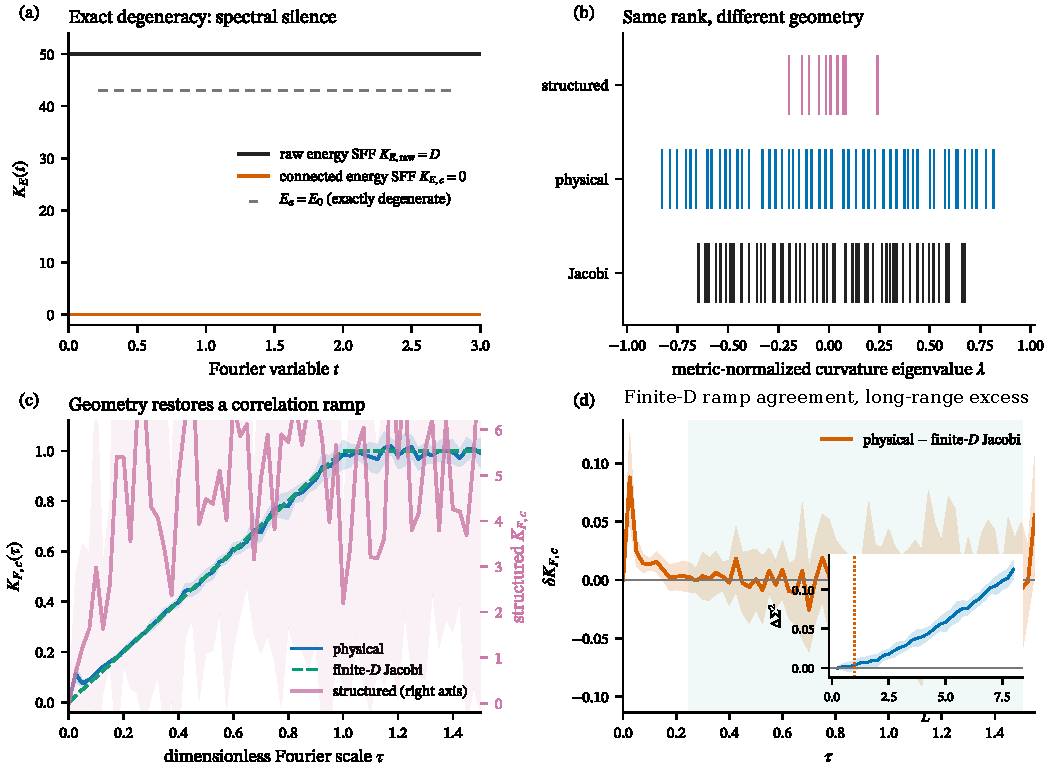
\includegraphics[width=\textwidth]{figures/figure_2_spectral_silence_v13.pdf}
  \caption{\label{fig:spectral}
  Spectral silence and resolved projector geometry.  (a) For the
  rank-$\SpectralFiberRank$ zero-mode manifold, whose audited bandwidth and
  external gap are $\SpectralKernelBandwidth$ and $\SpectralExternalGap$, the
  raw energy form factor is constant and its connected part vanishes.
  (b) Metric-normalized curvature spectra for a structured panel, a physical
  panel, and the finite-$D$ Jacobi reference at the same rank.  (c) The
  physical curvature form factor follows the registered finite-$D$ ramp,
  whereas the structured control does not.  (d) Physical-minus-reference
  residual; the inset shows the accumulated number-variance excess.  Shading
  denotes uncertainty from complete physical panels or registered
  finite-Jacobi draws, not independent curvature eigenvalues.
  }
\end{figure*}

\begin{figure*}[t]
  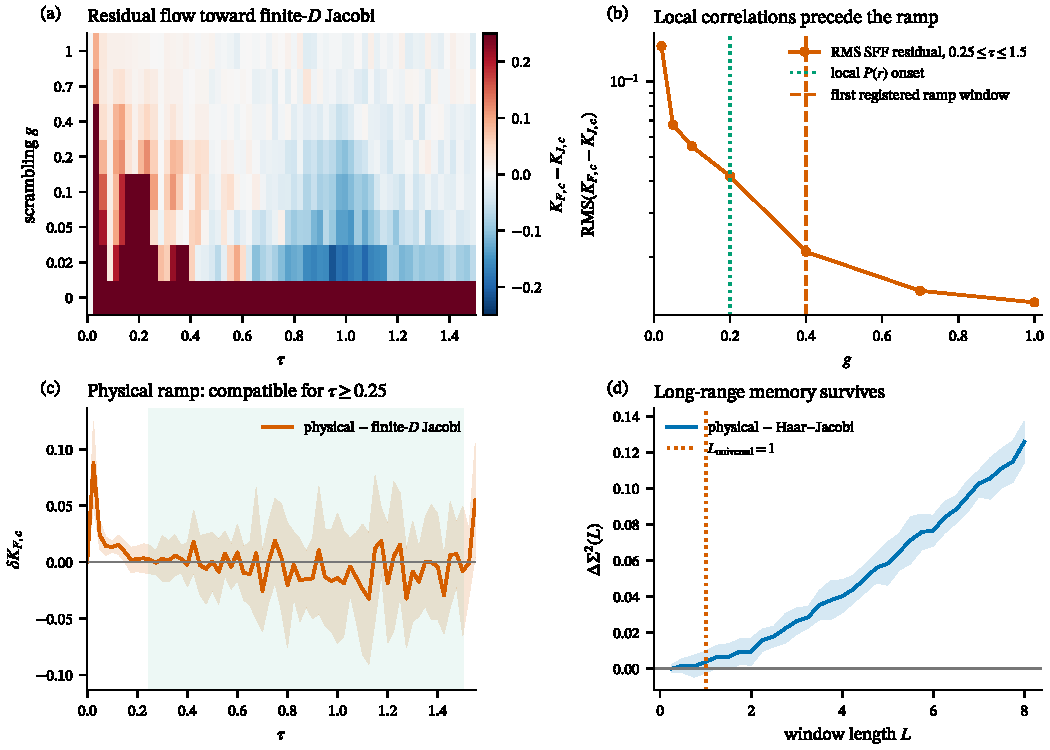
\includegraphics[width=\textwidth]{figures/figure_3_geometric_hierarchy_v13.pdf}
  \caption{\label{fig:hierarchy}
  Local-to-global hierarchy of curvature correlations.  (a) Difference
  between the physical and finite-$D$ Jacobi connected form factors versus
  Fourier scale $\tau$ and geometric-scrambling strength $g$.  (b) The local
  spacing-ratio criterion becomes compatible before the first registered
  ramp window.  (c) In that window the physical ramp residual is consistent
  with the finite-rank reference.  (d) The connected number-variance
  difference grows beyond the marked local scale, retaining long-range
  memory.  Curves and bands use a complete orbit or ensemble draw as the
  uncertainty unit; repeated $\tau$, window-length, and eigenvalue samples
  within one draw are not treated as independent.
  }
\end{figure*}

\begin{figure*}[t]
  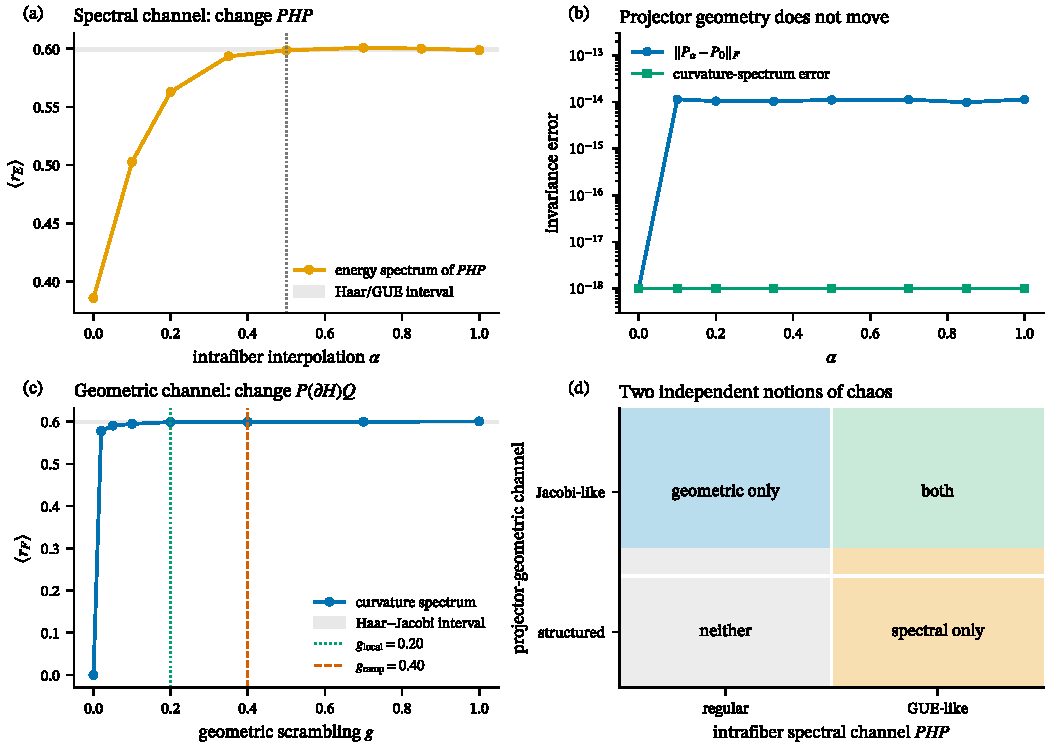
\includegraphics[width=\textwidth]{figures/figure_4_independent_channels_v13.pdf}
  \caption{\label{fig:channels}
  Independently controllable spectral and geometric channels.  (a) An
  intrafiber interpolation changes $PHP$ and brings its gap statistic to the
  registered Haar/GUE interval.  (b) The projector and curvature spectrum
  remain fixed to numerical precision during that intervention.  (c) A
  separate off-fiber interpolation changes $P(\partial H)Q+\mathrm{H.c.}$ and
  brings the curvature statistic to its Haar--Jacobi interval without using
  the intrafiber interpolation.  (d) The two axes permit structured,
  spectral-only, geometric-only, and jointly compatible regimes.
  Uncertainty bands are formed from the registered interpolation-endpoint
  ensemble.  \emph{Independent} here means separately tunable response
  channels, not independent entries of one response matrix.
  }
\end{figure*}

\begin{figure*}[t]
  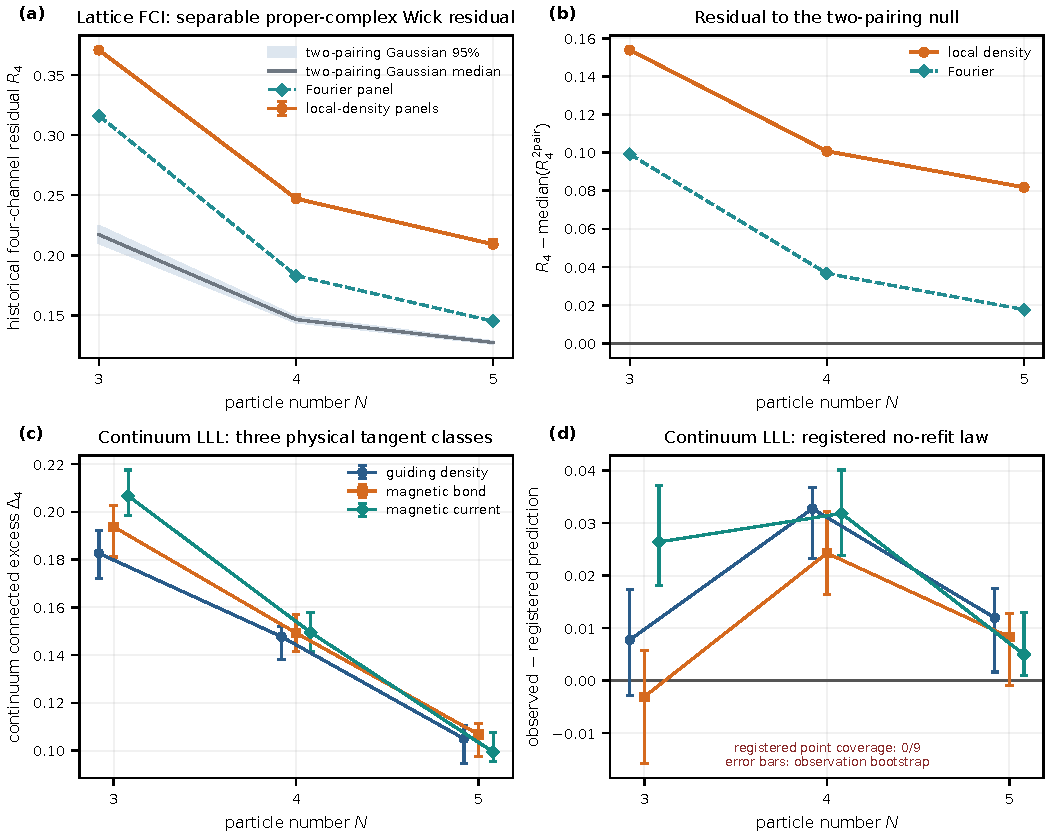
\includegraphics[width=\textwidth]{figures/figure_5_wick_parent_dependence_v13.pdf}
  \caption{\label{fig:wick}
  Restricted Wick residuals and parent dependence.  (a) Kapit--Mueller
  local-density and Fourier panels compared through the historical
  two-pairing residual under a separable proper-complex Gaussian null.
  (b) Residual relative to that two-pairing median.  This is not the corrected
  complete cumulant, which
  requires the full covariance, pseudocovariance, and all three complex Wick
  pairings.  (c) Continuum-LLL connected excess for guiding-density,
  magnetic-bond, and magnetic-current panels; error bars bootstrap complete
  physical panels.  (d) Observed-minus-predicted residual for the sealed
  no-refit common-plateau law.  The registered point coverage is zero of nine.
  This rejects that law across the displayed classes and sizes; it does not
  reject finite-size decay or all refitted forms.  The two parents are not
  pooled into one uncertainty estimate.
  }
\end{figure*}

\section{Spectral silence and geometric correlations in Laughlin manifolds}
\label{sec:laughlin-results}

\subsection{A degenerate spectrum with a resolved projector response}

We begin with the obstruction that motivates the geometric calculation.  In
the registered spectral-silence instance, the zero-mode projector has rank
$D=\SpectralFiberRank$.  Its numerical bandwidth is
$\SpectralKernelBandwidth$, whereas the first state outside the fiber lies at
the positive gap $\SpectralExternalGap$.  The former is a residual audit and
the latter is the scale that permits a reduced resolvent; neither is obtained
by unfolding a narrow band.  Within the accepted fiber all energies are
exactly equal at the algebraic parent, up to the reported solver residual.

The energy form factor consequently contains no information about the
orientation of $P$.  With the normalization used in Fig.~\ref{fig:spectral},
the raw contribution is the constant rank $D$, and the connected energy
spectral form factor vanishes.  This remains true for every tangent panel
because the energy calculation uses only the repeated eigenvalue.  It does not
imply a vanishing response: the same projector has nonzero
$X_a=Q(\partial_aP)P$ under the registered constraint or local-potential
tangents.

Figure~\ref{fig:spectral}(b) makes this separation visible without invoking a
single scalar summary.  A structured curvature, a physical curvature panel,
and a finite-$D$ Jacobi reference can have the same matrix rank while having
clearly different eigenvalue configurations.  The physical spectrum fills
the allowed interval and shows local repulsion, whereas the structured
control occupies a much smaller set.  Rank and exact energy degeneracy are
therefore insufficient to determine the curvature point process.

The curvature form factor provides a second comparison.  Over the registered
finite-$D$ window, the physical curve follows the Jacobi reference ramp within
the uncertainty obtained from complete reference draws.  At longer scales the
difference need not remain small.  Figure~\ref{fig:spectral}(d) and
Fig.~\ref{fig:hierarchy}(d) show the surviving form-factor and number-variance
residuals.  We describe this as finite-rank ramp agreement with long-range
memory.  The statement is tied to the displayed rank, normalization, and
tangent ensemble; it is not an asymptotic or universal claim.

\subsection{The order in which correlations appear}

To separate local and mesoscopic scales, the registered interpolation varies
the strength $g$ of the geometric scrambling while leaving the comparison
protocol fixed.  Figure~\ref{fig:hierarchy}(a) plots the curvature-form-factor
residual over Fourier scale and $g$.  The residual becomes small first in a
restricted interval of Fourier scales.  This flow is not uniform: a local
spacing criterion becomes compatible with the finite-$D$ reference before
the first registered ramp window appears, as summarized in
Fig.~\ref{fig:hierarchy}(b).

The ordering is physically useful.  Nearest-neighbor repulsion tests only the
shortest correlations of the curvature eigenvalues.  A ramp requires
correlations across a wider part of the point process, and number variance
integrates correlations over a still longer window.  Agreement of the first
statistic thus need not force agreement of the other two.  In the physical
panel, the registered ramp residual becomes compatible with the finite-$D$
reference over the shaded window in Fig.~\ref{fig:hierarchy}(c), while the
number-variance difference grows beyond the marked local scale in panel (d).

The uncertainty unit changes with neither Fourier time nor window length.  A
complete physical orbit or a complete ensemble draw is one realization; the
many eigenvalues and time samples within it are correlated observations.  In
particular, treating every curvature eigenvalue as an independent sample
would artificially narrow the bands in Figs.~\ref{fig:spectral} and
\ref{fig:hierarchy}.  The complete physical panel is the statistical unit
throughout this local-to-global comparison.

This hierarchy supplies the precise sense in which the geometry is
Jacobi-like.  It refers to local repulsion and a registered finite-rank ramp,
not to equality of the entire joint distribution with an invariant ensemble.
The long-range residual is evidence that the response retains information
about its physical construction after the local spectrum has become
compatible with the reference.

\subsection{Intrafiber and off-fiber interventions}

The separation between energy and geometry can also be imposed rather than
inferred.  Figure~\ref{fig:channels} compares two interventions on the same
block decomposition.  The intrafiber interpolation changes $PHP$.  Its level
statistics approach the registered GUE interval, but the projector is held
fixed.  The norm $\lVert P_\alpha-P_0\rVert_F$ and the curvature-spectrum
error remain at numerical zero, so this operation changes the spectral
channel without moving the quantum geometry.

The complementary interpolation changes the off-fiber block
$P(\partial H)Q+\mathrm{H.c.}$ while leaving the intrafiber intervention
absent.  The curvature gap statistic rapidly enters its Haar--Jacobi
reference interval.  Thus intrafiber spectral scrambling and off-fiber
projector motion are independent response channels.  Here
\emph{independent} means independently controllable in the block
intervention; it does not mean that estimators measured from one physical
panel are independent random variables.

The four quadrants in Fig.~\ref{fig:channels}(d) are therefore all logically
possible: neither channel may be random-matrix-like, either one can be
compatible while the other remains structured, or both can be compatible.
An exactly degenerate parent begins with a silent intrafiber spectrum, but it
is not forced into the geometrically structured quadrant.  This constructed
control also prevents us from interpreting agreement in the curvature
spectrum as indirect evidence that an unmeasured energy spectrum has become
chaotic.

\subsection{Historical Wick residual and the complete-cumulant boundary}

We next turn from curvature eigenvalues to response matrix elements.  The
Kapit--Mueller calculations use particle numbers $N=3,4,5$, with the audited
quantities collected here to expose the finite-size range:
\begin{table}[b]
\caption{\label{tab:laughlin-matrix}
Kapit--Mueller zero-mode ranks, external gaps, and the historical
four-channel residual.  Every number is supplied by the generated v13
registry macros.  The last two columns refer to the restricted separable
proper-complex two-pairing null, not to the corrected complete cumulant.}
\begin{ruledtabular}
\begin{tabular}{ccccc}
$N$ & $D$ & $\Delta$ & $R_4^{\rm 2pair}$ &
$R_4^{\rm 2pair}-R_{4,\mathrm{Wick}}^{\rm 2pair}$ \\
\hline
$3$ & \LaughlinNThreeRank & \LaughlinNThreeExternalGap
& \LaughlinNThreePhysicalTwoPairRFour & \LaughlinNThreeFourthMomentExcess \\
$4$ & \LaughlinNFourRank & \LaughlinNFourExternalGap
& \LaughlinNFourPhysicalTwoPairRFour & \LaughlinNFourFourthMomentExcess \\
$5$ & \LaughlinNFiveRank & \LaughlinNFiveExternalGap
& \LaughlinNFivePhysicalTwoPairRFour & \LaughlinNFiveFourthMomentExcess \\
\end{tabular}
\end{ruledtabular}
\end{table}
The corresponding Fock-space dimensions are
\LaughlinNThreeBasisDimension, \LaughlinNFourBasisDimension, and
\LaughlinNFiveBasisDimension.  Kernel count, gap, gauge invariance, leakage,
and resolvent gates pass for each row before the matrix statistic is formed.

The statistic in Table~\ref{tab:laughlin-matrix} and
Figs.~\ref{fig:wick}(a,b) is historical.  Its Gaussian null assumes a
separable covariance and a proper complex response, for which the
pseudocovariance pairing is set to zero.  It consequently subtracts two Wick
pairings.  The physical local-density panels and the structured Fourier panel
lie above that restricted null over the registered sizes.  Their residuals
decrease with $N$, as do the generated excesses in the last column.

This is a valid rejection of the stated restricted null, but it is not the
corrected complete cumulant of Eq.~\eqref{eq:wickresidual}.  A positive
historical two-pairing residual can be produced by nonseparable two-point
covariance or nonzero pseudocovariance without any connected four-point
cumulant.  We therefore do not call Figs.~\ref{fig:wick}(a,b) a detection of
non-Gaussian closure failure.  A corrected claim would require the full entry
covariance, all three complex Wick pairings, and uncertainty over declared
independent units.  The Laughlin row in Table~\ref{tab:model-evidence} records
that this complete-covariance gate has not been tested.

The physical error bars in Fig.~\ref{fig:wick}(a) use
\RawMomentResidualRealizationCount\ complete local-density panels.  One entire panel,
not one entry of $X_a$ or one pair of indices, is resampled.  The Fourier
panel is shown as a structured comparison and is not pooled with the local
panels to manufacture an uncertainty estimate.

\subsection{Parent dependence within two-body clustering}

The continuum lowest-Landau-level calculation preserves the same two-body
Laughlin constraint mechanism but changes the microscopic orbitals and the
realization of the physical tangents.  Figure~\ref{fig:wick}(c) displays
guiding-density, magnetic-bond, and magnetic-current panels separately.  For
the size-indexed registry branch, the exported connected excesses are
\ContinuumLaughlinNThreeConnectedExcess,
\ContinuumLaughlinNFourConnectedExcess, and
\ContinuumLaughlinNFiveConnectedExcess.  The figure, rather than those three
representative macros, resolves the full operator-class dependence and its
complete-panel bootstrap interval.

The comparison between the Kapit--Mueller and continuum LLL parents is
deliberately not a pooled test.  Both possess a positive factorized
$V_0$ parent and the same exact constraint-transport identity, but their
complement spectra and local generator maps differ.  Agreement would have
supported a parent-insensitive scalar law within this protection mechanism;
the registered outcome instead selects parent dependence.

Specifically, the sealed common-plateau prediction was evaluated without
refitting on the three continuum tangent classes and three registered sizes.
Figure~\ref{fig:wick}(d) reports that zero of nine registered predictions
cover their corresponding observed points.  The error bars there are
complete-panel observation-bootstrap intervals; the registered prediction is
not adjusted after seeing the continuum outcomes.

The no-refit failure has a narrow meaning.  It rejects that particular scalar
law as a simultaneous description of the displayed operator classes and
sizes.  It does not imply the absence of finite-size decay: all three
continuum classes decrease over the shown range.  It also does not show that
no refitted function could describe the data, that the two microscopic
parents occupy different phases, or that two-body clustering lacks a common
local curvature regime.  The result is parent and operator dependence of the
tested four-channel observable at finite rank.  It supplies no universality
or asymptotic conclusion.


\begin{figure*}[t]
  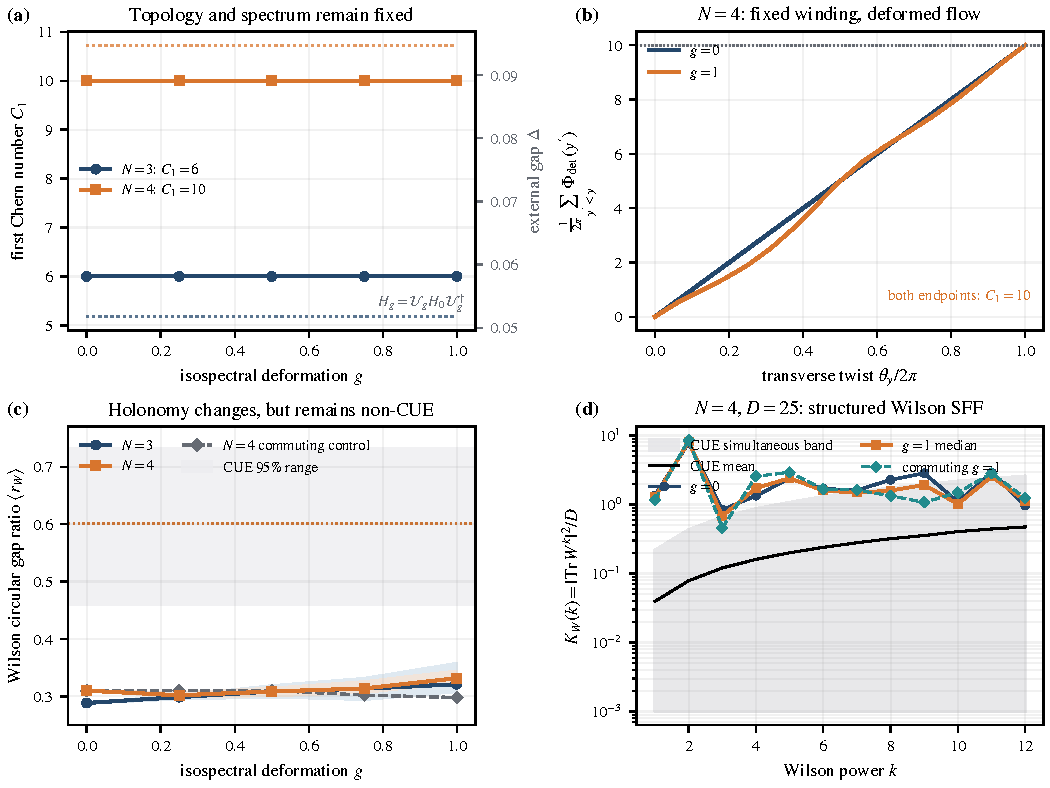
\includegraphics[width=\textwidth]{figures/figure_6_fixed_chern_holonomy_v13.pdf}
  \caption{\label{fig:holonomy}
  Non-Abelian holonomy along an exactly isospectral, fixed-Chern transport.
  (a) The ranks, first Chern numbers, and positive external gaps remain fixed
  under ambient unitary deformation.  (b) For
  $N=4$, $D=\HolonomyNFourRank$, the determinant Wilson-loop flow deforms
  while retaining winding $\HolonomyNFourChernNumber$.  (c) The internal
  Wilson gap ratio changes for noncommuting generators, while the commuting
  control remains structured; neither endpoint enters the CUE reference band.
  (d) The normalized Wilson form factor likewise retains non-CUE peaks.
  Marker intervals use the registered generator ensemble, and the gray CUE
  uncertainty bands use independent circular-unitary reference draws.
  Topology and the exact energy spectrum are unchanged throughout.
  }
\end{figure*}

\section{Geometry and topology at fixed Chern class}
\label{sec:topology}

The local curvature statistics studied above do not determine the topology of
the protected bundle, and the converse is also false.  To separate these
levels, we transport the Laughlin constraint map over the boundary-twist torus
$(\theta_x,\theta_y)$ while applying a periodic ambient unitary deformation
of strength $g$.  At every twist and every accepted $g$,
\[
 H_g(\boldsymbol\theta)
 =\mathcal V_g(\boldsymbol\theta)
 H_0(\boldsymbol\theta)
 \mathcal V_g^\dagger(\boldsymbol\theta).
\]
This is an exactness-preserving path rather than a fixed-parent probe.  The
many-body spectrum is identical point by point on the twist torus, the
protected rank stays fixed, and the external gap never closes.

\subsection{Fixed rank, gap, and first Chern number}

The two registered bundles have ranks \HolonomyNThreeRank\ and
\HolonomyNFourRank.  Their minimum gaps over the twist mesh and deformation
family are respectively \HolonomyNThreeMinimumGap\ and
\HolonomyNFourMinimumGap.  In addition to checking the kernel residual at
each vertex, we require the smallest singular value of every neighboring-frame
overlap to exceed \HolonomyNThreeMinimumOverlapSingularValue\ for the first
bundle and \HolonomyNFourMinimumOverlapSingularValue\ for the second.  These
overlap floors exclude a mesh on which the polar parallel transport becomes
ill-conditioned.

The determinant line bundle is unchanged along the deformation.  The
discretized trace curvature gives first Chern numbers
\HolonomyNThreeChernNumber\ and \HolonomyNFourChernNumber\ for the two ranks,
with the same integers on the primary and convergence meshes.
Figure~\ref{fig:holonomy}(a) shows these constants together with the open
external gaps.  The computation also compares the determinant Wilson-loop
phase with the integrated trace curvature; their agreement is a gauge
invariant check that the mesh winding and the plaquette Chern calculation
refer to the same Abelian sector.

Panel (b) illustrates this constraint for the rank-\HolonomyNFourRank\
bundle.  The determinant phase flow changes shape between the endpoints, but
its net winding remains \HolonomyNFourChernNumber.  Thus topology fixes the
integer winding, not its distribution along the transverse twist.  The same
distinction appears already at the level of local curvature: matrices can
redistribute their traceless part while preserving the integral of
$\Tr F_{\theta_x\theta_y}$.

\subsection{Non-Abelian holonomy inside a fixed topological sector}

For each fixed transverse twist, the polar factors of adjacent frame overlaps
are multiplied around the $\theta_x$ cycle to form a Wilson matrix
$W_x(\theta_y)$.  A frame change conjugates $W_x$, so its eigenphases, gap
ratio, and normalized spectral form factor are gauge invariant.  The
determinant of $W_x$ probes the Abelian winding discussed above; relative
eigenphases probe the internal $SU(D)$ holonomy.

The internal holonomy changes under noncommuting ambient generators even
though the energy spectrum and Chern number do not.  The median Wilson gap
ratio moves from \HolonomyNThreeBaseGapRatio\ to
\HolonomyNThreeFinalGapRatioMedian\ in the rank-\HolonomyNThreeRank\ bundle
and from \HolonomyNFourBaseGapRatio\ to
\HolonomyNFourFinalGapRatioMedian\ in the rank-\HolonomyNFourRank\ bundle.
The registered generator ensemble, rather than individual Wilson
eigenphases, is the uncertainty unit in this comparison.

This change is statistically resolved relative to its generator-to-generator
spread, but it does not carry the Wilson spectrum to the circular unitary
ensemble (CUE).  Figure~\ref{fig:holonomy}(c) places the endpoint gap ratios
below the CUE reference band, and panel (d) shows that the Wilson form factor
retains pronounced structured peaks.  The largest registered deformation is
therefore not CUE-compatible.  The commuting-generator control remains near
the undeformed curve, confirming that the observed change uses the
noncommuting part of the transport rather than the Chern calculation or an
uncontrolled change of spectrum.

The result has two immediate consequences.  First, a fixed first Chern number
does not fix the non-Abelian holonomy.  Bundles with the same rank, energy
spectrum, external gap, and Chern integer can have distinguishable internal
Wilson spectra.  Second, changing the holonomy within that sector does not by
itself produce Haar statistics.  Topological protection supplies the bundle
on which the geometric observable is defined; it neither forbids internal
mixing nor guarantees random-matrix closure.

The isospectral construction is important for this interpretation.  Had the
gap or protected rank changed with $g$, the holonomy shift could have been
attributed to a changing spectral cluster.  Had only a fixed-parent tangent
been evaluated, there would be no finite exactly degenerate bundle on which
to define the closed Wilson loop.  Here the equality
$H_g=\mathcal V_gH_0\mathcal V_g^\dagger$ holds over the complete twist torus,
so the difference between Abelian topology and non-Abelian geometry is
measured within one exact transported family.

Gauge covariance is checked separately from mesh convergence.  Random
unitaries applied to every local frame change individual link matrices but
leave the Chern integer and Wilson eigenphases invariant.  Increasing the
twist mesh reproduces the accepted integers and endpoint winding, while the
overlap singular-value gate controls the stability of the polar factors.
These checks matter because a smooth-looking eigenphase flow can otherwise
hide a branch-cut or coarse-mesh error.  The reported holonomy change survives
all three tests: random frame rotation, mesh refinement, and an open external
gap.

These two finite-rank bundles do not define a large-$D$ sequence.  The Chern
integers also differ between the two particle numbers, so they cannot be used
as evidence for size-independent Wilson statistics at a single fixed
topological charge.  What is established is a controlled counterexample to
the implication that a fixed Chern class fixes internal holonomy.  Testing an
asymptotic geometric law at fixed topology would require a growing-rank
sequence with the same topological sector, tangent prescription, mesh
convergence criteria, and independent generator ensemble.


\begin{figure*}[t]
  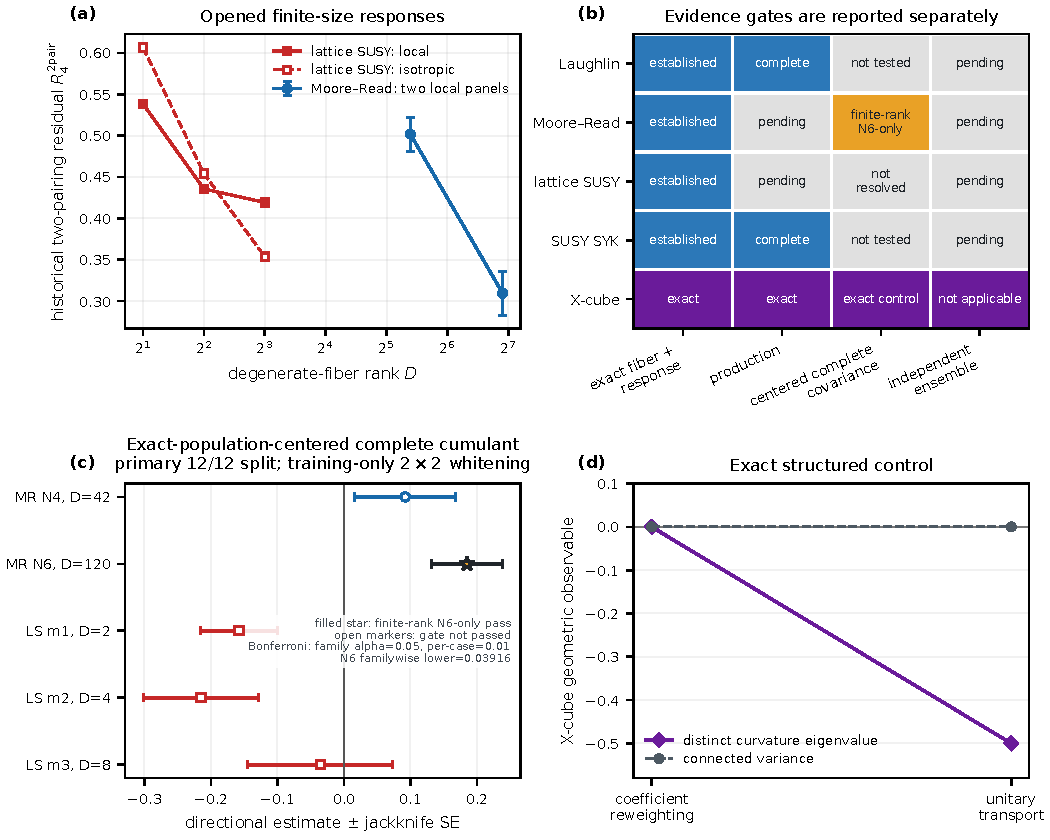
\includegraphics[width=\textwidth]{figures/figure_7_cross_mechanism_v13.pdf}
  \caption{\label{fig:mechanisms}
  Mechanism-resolved response under exact degeneracy.  (a) historical
  two-pairing residual $R_4^{2\mathrm{pair}}$ for local and isotropic lattice
  SUSY panels and two local Moore--Read panels.  This statistic uses a
  separable proper-complex null and is not the corrected complete cumulant.
  (b) Evidence cells are kept separate: exact fiber and nonzero response,
  production status, centered complete covariance, and an independent
  model/operator ensemble are different gates.  (c) Directional estimates
  of the exact-population-centered complete cumulant use a frozen 12/12
  split, training-only $2\times2$ channel whitening, all three Wick pairings,
  and delete-one-panel errors.  The filled star marks the sole familywise
  finite-rank pass, Moore--Read $N=6$; open markers do not pass.  The reverse
  split is descriptive and not pooled.  (d) X-cube coefficient reweighting
  has zero curvature, whereas local unitary transport has deterministic
  scalar curvature and zero connected variance.  These are exact structured
  controls, not Gaussian samples.
  }
\end{figure*}

\section{Three-body clustering and cohomological response}
\label{sec:cohomology}

Figure~\ref{fig:mechanisms} compares three protected constructions for which
the response is nonzero: a three-body clustering kernel, a random
supercharge, and a local lattice supercharge.  The common feature is an
exactly degenerate zero-energy fiber separated from its complement.  The
origin of that fiber and the sampling measure are different.  We therefore
compare the algebra and the statistical result within each model before
placing their evidence cells next to one another.  In particular, a tangent
panel at one fixed Hamiltonian is not interchangeable with an independent
disorder realization.

\subsection{Moore--Read: an exact moving kernel}

The Moore--Read parent is a sum of positive three-particle constraints,
Eq.~\eqref{eq:moore-read-parent}.  The states in its kernel obey the same
three-body clustering condition at exactly zero energy
\cite{mooreread1991,zhang2023parent}.  For the fixed-four-quasihole sequence
$N_\phi=N+2$, the two opened systems have $(N,D)=(4,
\MooreReadNFourRank)$ and $(6,\MooreReadNSixRank)$.  The first positive
energies, \MooreReadNFourExternalGap\ and
\MooreReadNSixExternalGap, respectively, verify that the response is taken
for an isolated projector rather than for a numerically selected portion of
a continuum.

The guiding-density directions are an exactness-preserving generator
transport.  If $G_a$ is lifted to the $N$-particle Fock space by
$\Gamma_N(G_a)$, differentiation of the transported constraint gives
\begin{equation}
 (\partial_aH)P=-H\Gamma_N(G_a)P,
 \qquad
 X_a=Q\Gamma_N(G_a)P.
 \label{eq:mr-generator-response}
\end{equation}
Thus $S_a=P(\partial_aH)P=0$, while the off-fiber block $X_a$ is generally
nonzero.  This identity is checked against the parent action and complement
leakage for every stored panel.  It matters conceptually: the response is not
the derivative of a multiplet that immediately splits.  It is the derivative
of an exactly degenerate kernel that moves under a finite invertible
constraint path.

The finite-size calculations used two related, but inequivalent, fourth-order
statistics.  The historical two-pairing residual in
Fig.~\ref{fig:mechanisms}(a) subtracts a separable proper-complex Gaussian
prediction.  Its local-panel medians are
\MooreReadNFourLocalTwoPairRFour\ and
\MooreReadNSixLocalTwoPairRFour; the structured-line controls are
\MooreReadNFourStructuredTwoPairRFour\ and
\MooreReadNSixStructuredTwoPairRFour.  Those values describe the old
$R_4^{2\mathrm{pair}}$ observable.  They neither include the
pseudocovariance pairing nor reproduce an arbitrary entrywise covariance, so
they are not a test of the complete Gaussian law.

The v12 raw, uncentered three-pairing calculation is also retained only for
provenance.  Its response arrays were neither population-centered nor
channel-whitened before the moment subtraction.  The corresponding raw
estimates, \MooreReadNFourRawMomentResidualEstimate\ and
\MooreReadNSixRawMomentResidualEstimate, cannot be interpreted as connected
cumulants.  A nonzero raw value may contain the finite-population mean and is
therefore claim-ineligible even when a nominal normal-reference probability
is small.  Figure~\ref{fig:mechanisms}(b) marks this distinction explicitly:
``exact fiber and response'' and ``centered complete covariance'' are
separate evidence questions.

For the corrected $R_4^{\mathrm{full}}$ calculation, one fixed-base tangent
panel is the statistical unit.  Each system has a registered finite
population of torus guiding-density anchors, and linearity gives its exact
population mean before any panels are assigned to inference.  The mean
vanishes for the uniform traceless guiding-density population; it is not
estimated from the observed inference half.  The \FullRFourTrainingCount\
panels in the training half determine only the $2\times2$ channel Gram
matrix.  Its inverse square root is then frozen and applied to the disjoint
\FullRFourInferenceCount\ panels.  We refer to this as the frozen 12/12
split.  The training half alone fixes the whitening transformation.  All
three Wick pairings, including the pseudocovariance term, are subtracted from
the inference-panel U-statistic.

Uncertainty is obtained by deleting one complete inference panel and
recomputing the contraction.  The registered scalar direction is tested with
a Student-$t$ reference with \FullRFourStudentTDegreesOfFreedom\ degrees of
freedom.  A Bonferroni correction controls the family level
\FullRFourFamilyAlpha\ across five registered primary cases
(\FullRFourPrimaryFamilySize\ in total), giving per-case level
\FullRFourPerCaseAlpha.  This protocol
is conditional on exchangeability of the fixed-base panels; it is not an
estimate over Moore--Read Hamiltonians or over parent-Hamiltonian families.

At $N=4$, $D=\MooreReadNFourRank$, the directional estimate is
\MooreReadNFourFullRFourDirectionalEstimate, while the familywise one-sided
lower bound is \MooreReadNFourFullRFourFamilywiseLower.  The registered
positive-direction gate does not pass.  At $N=6$,
$D=\MooreReadNSixRank$, the corresponding estimate is
\MooreReadNSixFullRFourDirectionalEstimate\ and the familywise lower bound is
\MooreReadNSixFullRFourFamilywiseLower; this case passes.  The positive cell
in Fig.~\ref{fig:mechanisms}(c) is consequently a finite-rank $N=6$ result.
It is not an asymptotic statement, and the absence of a pass at $N=4$ forbids
a monotone scaling claim from these two ranks alone.  The reverse split is
descriptive and is not pooled with the primary split, even where its point
estimate has the same sign.

This result establishes a connected fourth-order response contraction at
one rank for the stated tangent population after complete covariance and
pseudocovariance subtraction.  It does not establish that all fourth-order
components are nonzero, that the effect persists with $D$, or that different
three-body parents share the same law.  It also does not identify a dynamical
Lyapunov exponent: the measured object is the geometry of an exactly
degenerate projector over coupling space.

There are two further reasons not to read the $N=4,6$ comparison as a fit.
First, the ambient occupation-space dimensions and the protected ranks change
together, so a change in the scalar contraction cannot be assigned uniquely
to $D$.  Second, the response channels are generated by a discrete torus
population whose geometry also changes with $N_\phi$.  An asymptotic test
would have to hold the operator prescription fixed in physical units, open
additional ranks, and preregister the scaling quantity before examining the
new outcomes.  Here the two cases instead test whether the same finite-panel
protocol can be carried out at two nontrivial ranks and whether its familywise
gate is resolved in either one.

The fixed-base qualification does not contradict exact transport.  Every
$G_a$ defines a finite isospectral constraint path, but the collection of
panels is evaluated at the same base parent and base projector.  The
jackknife therefore samples the registered distribution of tangent
directions through one point of the projector bundle.  It does not sample
different points along a path, and it does not absorb the correlation among
channels within one panel into the sample count.  This distinction is why
the full response tensor of a panel, rather than each generator or matrix
entry, is deleted in the uncertainty calculation.

\subsection{Random-supercharge cohomology}

The random supersymmetric model replaces a clustering ideal by a chain
complex.  A cubic nilpotent supercharge $Q$ maps a charge-$r$ sector to the
charge-$(r-3)$ sector, and
\begin{equation}
 H_r=Q_{r+3}Q_{r+3}^{\dagger}+Q_r^{\dagger}Q_r
 \label{eq:syk-hodge-laplacian}
\end{equation}
is its Hodge Laplacian.  Its zero modes are harmonic representatives of
$Q$-cohomology, $\ker Q_r/\operatorname{im}Q_{r+3}$, and hence are annihilated
by both $Q$ and $Q^\dagger$ \cite{fu2017susy}.  Exact degeneracy follows from
nilpotency and positivity, not from spatial locality.  This is the finite
supersymmetric sector in which non-Abelian Berry curvature was previously
proposed as a chaos probe \cite{chen2026}.

Let $\Pi_-=Q_{r+3}Q_{r+3}^{\dagger}H_r^+$ and
$\Pi_+=Q_r^{\dagger}Q_rH_r^+$ be the orthogonal projectors onto the exact and
coexact positive-energy subspaces, where $H_r^+$ is the Moore--Penrose inverse
of $H_r$ on the complement of its kernel.  Differentiating the two Hodge terms
then separates the response into $X_a^-=\Pi_-X_a$ and
$X_a^+=\Pi_+X_a$,
\begin{equation}
 X_a=X_a^{-}\oplus X_a^{+},
 \qquad
 \langle X_a^{-},X_b^{+}\rangle_{\mathrm{HS}}=0.
 \label{eq:hodge-response-split}
\end{equation}
Here the direct resolvent response and the sum of the two branch responses
are checked independently.  The branch weights, channel covariances, and
left/right covariance spectra can therefore be used to build a
Hodge-resolved Gaussian comparison without opening the fourth-order outcome.
This branch structure is physical information imposed by the complex; it
should not be discarded by replacing the full response with an isotropic
rectangular matrix.

The registered $N=14$ test used a complete independent disorder realization
as the uncertainty unit.  The adjacent- and central-charge sparse panels have
observed median historical residuals
\SusySykNFourteenMedianOne\ and
\SusySykNFourteenMedianTwo.  Before those outcomes were unsealed, the null
distribution was generated from the stored two-point Hodge signatures.  The
held-out medians lie outside both the collapsed and Hodge-resolved prediction
intervals.  This rejects the frozen separable proper-complex Gaussian null
for the registered response statistic.

The qualifier ``separable'' is essential.  That null matches marginal
channel, target, external, and exact/coexact covariance spectra, but it is not
the complete entrywise covariance $C$ together with pseudocovariance $\Pi$.
Consequently, its rejection can arise from a connected fourth cumulant or
from nonseparable two-point structure omitted by the null.  The random-SYK
cell for centered $R_4^{\mathrm{full}}$ remains not tested.  We do not use the
historical residual to claim complete-covariance non-Gaussianity, and we do
not pool its independent-realization bootstrap with the fixed-base panel
jackknife used for Moore--Read.

This separation also identifies the useful next test.  Random couplings
supply genuine Hamiltonian-to-Hamiltonian sampling, whereas the Moore--Read
calculation supplies an exact moving-kernel path at one parent.  A common
claim would require the same centered full-covariance observable and a
matched tangent prescription in both ensembles.  Those cells are absent from
the present registry.

The Hodge split also changes the meaning of apparent isotropy.  Unitary
rotations within the exact image and within the coexact image may leave all
stored covariance spectra invariant while changing correlations between the
two embedded subspaces and the protected fiber.  A collapsed null that keeps
only the total left and right spectra forgets even more information.  The
sealed v7 comparison was designed to ask whether these progressively richer
separable nulls predicted the held-out median.  Their failure is reproducible
evidence for covariance memory beyond those summaries; it is deliberately
not relabeled as the complete cumulant of Sec.~\ref{sec:statistics}.

\subsection{Local lattice cohomology}

The lattice construction retains the Hodge mechanism but changes both
locality and sampling.  On a union of $m$ six-site cycles, the nilpotent
supercharge acts on the independence complex, and its harmonic sector has
ranks $D=\LatticeSusyMOneRank$, \LatticeSusyMTwoRank, and
\LatticeSusyMThreeRank\ for $m=1,2,3$.  The corresponding positive gaps are
\LatticeSusyMOneExternalGap, \LatticeSusyMTwoExternalGap, and
\LatticeSusyMThreeExternalGap.  Local changes of the site couplings move the
harmonic projector.  The response again splits into exact and coexact
branches; their measured local-panel balance factors are
\LatticeSusyMOneHodgeBalance, \LatticeSusyMTwoHodgeBalance, and
\LatticeSusyMThreeHodgeBalance.  Thus the local family is neither a
fixed-projector control nor a single-branch rectangular ensemble.

Panel (a) shows the historical two-pairing residual for local and isotropic
tangents.  The local values
\LatticeSusyMOneLocalTwoPairRFour,
\LatticeSusyMTwoLocalTwoPairRFour, and
\LatticeSusyMThreeLocalTwoPairRFour\ differ from their isotropic counterparts
\LatticeSusyMOneIsotropicTwoPairRFour,
\LatticeSusyMTwoIsotropicTwoPairRFour, and
\LatticeSusyMThreeIsotropicTwoPairRFour.  These finite-size differences show
that the accessible tangent class matters.  As in Moore--Read, however, the
old $R_4^{2\mathrm{pair}}$ numbers do not answer the complete-covariance
question.  The v12 raw estimates are likewise uncentered and are not used for
a claim.

The corrected calculation uses the exact population mean obtained by
enumerating the registered ordered local-coordinate marginals.  This mean is
nontrivial because the discrete local-tangent construction is not symmetric
entry by entry.  After population centering, the same frozen 12/12 split,
training-only channel whitening, three-pairing U-statistic, Student-$t$
reference, and five-case Bonferroni family are used.  This alignment makes the
Moore--Read and lattice rows comparable at the level of the estimator, but it
does not turn the lattice panels into independent graph realizations.

Disjoint cycle components make the algebraic rank sequence exactly auditable,
but they also impose a tensor-product ancestry on the cohomology.  Increasing
$m$ simultaneously adds degrees of freedom and repeats a local building
block.  The sequence is therefore useful for checking how a known branch
structure enters the response and the estimator; it is not a connected-
lattice thermodynamic sequence.  A claim of locality-driven universality
would require connected graphs, a matched local tangent density, and an
independent ensemble at each size.  None of those missing conditions can be
replaced by treating the many coordinate pairs at one graph as independent
Hamiltonians.

The primary directional estimates are
\LatticeSusyMOneFullRFourDirectionalEstimate,
\LatticeSusyMTwoFullRFourDirectionalEstimate, and
\LatticeSusyMThreeFullRFourDirectionalEstimate.  Their familywise lower
bounds are \LatticeSusyMOneFullRFourFamilywiseLower,
\LatticeSusyMTwoFullRFourFamilywiseLower, and
\LatticeSusyMThreeFullRFourFamilywiseLower.  None of the three registered
positive-direction gates passes; failure of the positive-direction gate does
not prove Gaussianity.  It supplies neither an equivalence test nor a
two-sided upper bound on every component of $\mathcal K$.  A negative point
estimate in a preselected direction may coexist with a nonzero cumulant in a
different direction, and a small finite panel family may lack power.  The
reverse split is descriptive here as well.

The appropriate conclusion is therefore asymmetric.  Local lattice
cohomology supports an exact, moving, branch-reducible projector with
nontrivial response, but the registered positive full-cumulant contraction is
not resolved for $D=\LatticeSusyMOneRank,
\LatticeSusyMTwoRank,\LatticeSusyMThreeRank$.  Moore--Read resolves that
contraction only in the displayed rank-\MooreReadNSixRank\ case.  Random
supercharge SYK rejects a narrower separable null using independent disorder
realizations, while its complete entrywise-covariance cell remains open.
These are three different statements, not three measurements of a universal
number.

\section{Stabilizer counterexamples}
\label{sec:stabilizer}

The X-cube model provides an exact control in which the protected rank grows
rapidly but the quantum geometry is fully determined by the tangent algebra.
On the three-torus its dependent stabilizer relations leave $6L-3$ logical
qubits and ground-space dimension $2^{6L-3}$
\cite{vijay2016xcube}.  Neither a large $D$ nor a moving projector is therefore
sufficient to produce random-matrix curvature.  Figure~\ref{fig:mechanisms}(d)
shows two deformations that separate these possibilities without allocating
the exponentially large ground-space matrix.

The calculation is performed in the binary symplectic representation.  Each
Pauli stabilizer is a row $(\bm x|\bm z)$ over $\mathbb F_2$, commutation is a
symplectic inner product, and row reduction determines the number of
independent constraints.  This proves the logical-qubit count without
diagonalizing a $2^{3L^3}$-dimensional Hamiltonian.  It also exposes the
relation responsible for the transported curvature: the ordered product of
the chosen local generators is reduced against the stabilizer row space,
rather than inferred from a small-system spectrum.

\subsection{Positive coefficient reweighting}

First vary the positive coefficients multiplying the commuting stabilizers
while keeping the Pauli generators fixed.  The simultaneous $+1$ eigenspace
does not depend on those coefficients as long as none crosses zero.  Hence the
projector is parameter independent,
\begin{equation}
 \partial_aP=0,
 \qquad X_a=0,
 \qquad g_{ab}=F_{ab}=0.
 \label{eq:xcube-flat-control}
\end{equation}
The registered coefficient reweighting curvature is exactly
\XCubeCoefficientCurvature.  This is stronger than a small numerical
residual: it follows from the common stabilizer eigenspace.  The deformation
changes excitation energies and may change the gap scale, yet it cannot
rotate the protected subspace.  Energy dependence outside the fiber and
geometry of the fiber are independent data.

This control also identifies the relevant failure boundary.  A coefficient
passing through zero removes one constraint and closes the corresponding
gap; a logical operator added within the ground space makes $PHP$ nonscalar
and splits the exact multiplet.  Neither operation belongs to the open,
constant-rank family of Eq.~\eqref{eq:xcube-flat-control}.

Generic local Pauli fields need not split the torus ground space at first
order because a detectable error maps it out of the code space.  Their
finite-size splitting appears only at the perturbative order at which a
noncontractible logical operator is assembled.  That exponentially or
high-order small splitting is physically important for code stability, but
it is distinct from exact degeneracy at the commuting-projector point.  Our
controls stay on paths for which the algebra certifies exact equality of all
ground energies.

\subsection{Local isospectral unitary transport}

The second deformation conjugates the full commuting-projector Hamiltonian
by local unitaries.  Let
\begin{equation}
 H(\lambda_1,\lambda_2)=UHU^\dagger,
 \qquad
 U=e^{-i\lambda_1G_1}e^{-i\lambda_2G_2}.
 \label{eq:xcube-unitary-transport}
\end{equation}
The spectrum, degeneracy, and gap are then preserved exactly, while
$P(\boldsymbol\lambda)=UPU^\dagger$ moves.  The registered local Pauli
generators are individually detectable, anticommute, and have an ordered
product equal to a stabilizer up to phase.  Their commutator therefore acts
centrally on the code space.  The curvature is nonzero but scalar,
\begin{equation}
 F_{12}=\XCubeTransportCurvatureEigenvalue\,P,
 \qquad
 D^{-1}\Tr\!\left[
   \bigl(F_{12}-D^{-1}\Tr(F_{12})P\bigr)^2
 \right]=\XCubeTransportConnectedVariance.
 \label{eq:xcube-scalar-curvature}
\end{equation}
The dense low-rank toy audit fixes the sign in
Eq.~\eqref{eq:xcube-scalar-curvature}; the production statement follows from
binary symplectic identities for every opened size.  Thus unitary transport
is exactly isospectral and geometrically nontrivial, but its non-Abelian
curvature contains no fluctuating eigenvalue sector.  Parallel transport
around an infinitesimal loop gives a common phase rather than relative
mixing within the code space.

Because the two generators anticommute, their ordered infinitesimal
transports do not cancel.  Because their product is a stabilizer, however,
the resulting commutator has the same action on every code state.  This is a
concrete example of noncommuting motion in the ambient Hilbert space whose
projection to the fiber lies in the center.  It rules out the converse
shortcut that any noncommuting deformation must generate a fluctuating
non-Abelian spectrum.

The scalar curvature is compatible with a nonzero metric: the projector can
move in the ambient Hilbert space even though the commutator of two accessible
motions becomes central after restriction to the fiber.  What vanishes is the
traceless curvature component used for level-repulsion and connected-variance
tests.  This distinction prevents a nonzero Berry phase from being mistaken
for stochastic non-Abelian mixing.

The connected variance vanishes because the response algebra collapses to
the center on the protected fiber.  There is no ensemble of fluctuating
curvature matrices to which a Jacobi or Gaussian comparison should be
applied.  The complete-covariance gate is not applicable to this exact
control; labeling it ``passed'' or ``failed'' would confuse deterministic
centrality with a statistical null.

Together, the two X-cube paths exclude two shortcuts in interpreting the
other models.  The flat path shows that exact degeneracy can coexist with no
projector response.  The unitary transport path shows that nonzero response
and curvature can coexist with zero connected variance.  Thus large exact
degeneracy is not sufficient for geometric chaos; one must also establish a
noncentral accessible response algebra and then test its statistics with an
appropriate sampling measure.

\section{Protection, mixing, and statistical classes}
\label{sec:classification}

The examples above suggest a classification with three logically independent
entries.  The \emph{protection class} records why a rank-$D$ multiplet is
exactly degenerate.  The \emph{mixing class} records which directions of the
Grassmannian are reached by the allowed Hamiltonian tangents.  The
\emph{statistical class} records the measure under which a statement about
those directions is made.  Keeping these columns separate is necessary:
protection does not determine mixing, and mixing at one base Hamiltonian does
not determine Hamiltonian-to-Hamiltonian statistics.

\subsection{Response algebra and commutant}

At a fixed protected projector define the accessible off-fiber space and its
fiber algebra by
\begin{align}
 \mathfrak X
 &=\operatorname{span}\{X_a\}
   \subset\operatorname{Hom}(P\cH,Q\cH),
 \nonumber\\
 \mathfrak A_X
 &=\operatorname{alg}\{X_a^\dagger X_b\}_{a,b}
   \subset\operatorname{End}(P\cH).
 \label{eq:response-algebra}
\end{align}
The response rank is the dimension of $\mathfrak X$ after exact tangent-null
directions are removed.  It measures the number of accessible projector
velocities, not the degeneracy $D$ itself.  The commutant
\begin{equation}
 \mathfrak C_X=\{M\in\operatorname{End}(P\cH):
 [M,A]=0\ \text{for all }A\in\mathfrak A_X\}
 \label{eq:response-commutant}
\end{equation}
records exact block structure invisible to an eigenvalue histogram of one
curvature matrix.  A large commutant signals conserved subblocks or repeated
representations.  A scalar algebra has the entire endomorphism algebra as its
commutant; an irreducible full matrix algebra has only the center.  These are
algebraic statements and should be established before a random-matrix law is
fitted.

The Hermitian curvature combination
$i(X_a^\dagger X_b-X_b^\dagger X_a)$ belongs to $\mathfrak A_X$.  Its
centrality is therefore another useful coordinate.  We distinguish a fixed projector ($\mathfrak X=0$), central
curvature ($F_{ab}\propto P$), structured or reducible response (nonzero
$\mathfrak X$ with an exact branch or block decomposition), and finite-size
stochastic response (noncentral matrices with measured ensemble
fluctuations).  The last label is empirical and rank-specific.  It does not
mean that $\mathfrak A_X$ has been proved to become a free or invariant random
algebra as $D\rightarrow\infty$.

\subsection{Protection class}

Constraint-kernel protection occurs when $H=C^\dagger C$ and the common
nullity of the constraints is constant.  The Laughlin and Moore--Read parents
fall in this class, with two- and three-body clustering conditions,
respectively.  Exactness-preserving transport rotates $C$ together with its
kernel; a generic fixed-parent perturbation can instead produce a nonscalar
$P(\partial H)P$ and split the fiber.  The same protection class consequently
permits both a finite exact path and a splitting probe, depending on the
tangent.

Cohomological protection occurs for a nilpotent $Q$ and
$H=\{Q,Q^\dagger\}$.  Harmonic representatives identify the zero modes with
$Q$-cohomology.  The random cubic supercharge and the independence-complex
lattice model share this origin, but their tangent spaces and sampling units
are not the same.  The Hodge decomposition adds an exact/coexact branch
structure to $\mathfrak X$.  A Gaussian comparison that ignores that branch
structure tests a different null from one that conditions on it.

Stabilizer protection follows from a commuting Pauli constraint algebra and
its dependent relations.  In X-cube, positive coefficient changes leave the
common eigenspace fixed, whereas unitary conjugation moves it isospectrally.
The protected rank is exponentially large in a linear system size, yet the
opened transport curvature remains central.  This example directly separates
the count of protected states from the complexity of their accessible
geometry.

A quasi-degenerate isolated cluster, such as the checkerboard replication,
belongs to none of these exact classes at finite size.  It can test whether a
geometric trend survives an internal bandwidth, but it cannot support the
algebraic spectral-silence statement used for an exact kernel.

\subsection{Mixing class}

The frozen class has $\partial_aP=0$.  X-cube coefficient reweighting is the
exact example; changing $PHP$ inside a fixed subspace can also alter spectral
statistics without changing the projector.  Such a tangent provides no
geometric chaos datum, regardless of $D$.

The central class has $X_a\neq0$ for some tangents but
$F_{ab}=f_{ab}P$ on the protected fiber.  X-cube unitary transport realizes
this case.  It produces a Berry phase density and can have a nonzero quantum
metric, but all states in the fiber see the same infinitesimal holonomy.  The
traceless curvature and its connected variance vanish.

The structured class has a noncentral response subject to a proper invariant
decomposition.  Local lattice SUSY supplies exact and coexact Hodge branches;
structured Laughlin and Moore--Read generator lines restrict the accessible
operator span.  Here a response rank alone is inadequate.  The commutant,
branch weights, and channel covariance must be retained in the null model.
Failure of a naive isotropic comparison can reflect omitted two-point
structure rather than a connected higher moment.

The stochastic class is assigned only when an ensemble of noncentral
responses has been measured.  The finite Laughlin panels, the Moore--Read
fixed-base panels, and random-supercharge realizations exhibit such
fluctuations under their registered protocols.  Their higher-order status is
not uniform: the rank-\MooreReadNSixRank\ Moore--Read case passes the centered
full-cumulant direction; the smaller Moore--Read and lattice cases do not;
SUSY SYK rejects a separable Hodge-Gaussian null but lacks a complete
entrywise-covariance test.  ``Finite-size stochastic response'' is therefore
a mixing description, not a universal closure claim.

\subsection{Statistical class and claim level}

Deterministic algebraic controls form the first statistical class.  Their
results---zero projector derivative, scalar curvature, or a vanishing
connected variance---follow from exact identities.  They need numerical
audits of implementation and sign, but no bootstrap population is created by
repeating eigenvalues inside the code space.

Fixed-base tangent populations form the second class.  Moore--Read and local
lattice SUSY use complete panels treated as exchangeable conditional on a
common Hamiltonian.  Exact finite-population centering and a training-only
whitener prevent the same inference panels from selecting their own null.
The resulting jackknife quantifies panel-to-panel variation at that base.  It
does not quantify variation across disorder, parent Hamiltonians, or
topological phases.

Independent disorder realizations form the third class.  The random
supercharge calculation samples the couplings anew, so one realization is a
Hamiltonian-level unit.  Its historical sealed prediction is stronger than a
same-Hamiltonian resampling statement, but its covariance null is narrower
than the full complex Gaussian law.  Statistical independence of the units
does not repair a misspecified covariance model.

Loop or moduli-space sampling forms a fourth class for global observables.
Wilson loops and Chern numbers compare transported frames over extended
parameter cycles.  Repeated mesh points on one loop are not independent
realizations, and the loop parameter is not physical time.  These global
objects can retain structure even when a local curvature statistic resembles
a finite random-matrix reference.

This classification fixes the order of a geometric-chaos claim.  One first
states the protection mechanism and verifies a constant-rank gap.  One then
specifies the tangent class, computes the response rank, and identifies the
commutant or branch structure of $\mathfrak A_X$.  Only after that does one
choose a statistical class, match the complete relevant two-point structure,
and test the higher-order status.  An asymptotic Geometric ETH would require
these ingredients along a growing-rank sequence with a fixed operator class
and controlled connected cumulants.  The independent model/operator ensemble
has not been established here, and the present finite-rank comparisons do not
supply that theorem.

\section{Discussion and limitations}
\label{sec:discussion}

\subsection{What the finite-rank comparison establishes}

The calculations answer a question that cannot be posed through ordinary
level statistics.  When a parent Hamiltonian has a rank-$D$ eigenspace pinned
to one energy, neither its zero spacings nor its spectral form factor
distinguishes a rigid projector from one that rotates strongly under local
changes of couplings.  The non-Abelian quantum geometric tensor resolves this
difference because it measures virtual excursions from the protected fiber
into the gapped complement.  The relevant randomness is therefore randomness
of the embedding $P(\boldsymbol\lambda)\subset\mathcal H$, not randomness of
the repeated eigenvalue $E_0$.

Across clustered Hall parents and cohomological kernels, the response is
nontrivial even though the protected energies remain equal at the accepted
base point or along an exact transported family.  Several finite-rank
curvature spectra display Jacobi-like local eigenvalue repulsion.  This is the
part of the result that most closely resembles an ordinary random-matrix
criterion: nearby curvature eigenvalues avoid one another after the
finite-$D$ density is treated correctly.  It is also the narrowest part of the
claim.  The comparison does not show that the full response matrix is drawn
from an invariant Jacobi ensemble.  Its channel covariance, pseudocovariance,
and exact/coexact or stabilizer branch structure remain visible at larger
scales.

We use \emph{geometric chaos} for this combination of noncommuting projector
response, stochastic local curvature correlations, and a nontrivial
complement channel.  The phrase does not assert that the parent Hamiltonian
thermalizes.  Indeed, the protected sector has no internal energy differences
on which a conventional ETH ansatz could act.  What is measured is the
sensitivity and correlation structure of the degenerate subspace under a
declared tangent ensemble.  This meaning is consistent with the use of
eigenstate deformation as a chaos-sensitive observable \cite{pandey2020} and
with the proposal to use Berry curvature inside BPS multiplets
\cite{chen2026}, while remaining agnostic about long-time relaxation.

\subsection{Protection, mixing, and the meaning of a tangent}

The separation between $S_a$ and $X_a$ is more than a bookkeeping device.
$S_a$ asks whether a perturbation resolves energies inside the fiber;
$X_a=Q(\partial_aP)P$ asks whether it changes the fiber's embedding.  An
exactly transported parent can have $S_a=0$ and large $X_a$, whereas a scalar
rescaling can have both responses trivial.  Conversely, an arbitrary local
potential can split the fiber and rotate its spectral cluster at the same
time.  Calling all three operations \emph{deformations of the parent} would
erase the physical distinction on which the geometric test rests.

Accordingly, finite-path claims in this work come only from
exactness-preserving transport.  For the Laughlin and Moore--Read generator
panels, the constraint map is transported unitarily, the kernel rank remains
fixed, and the differentiated identity gives $S_a=0$.  Closed paths can then
support a Wilczek--Zee holonomy \cite{wilczekzee1984}; its non-Abelian part
contains information not fixed by the first Chern number.  In a gapped
topological phase, quasiadiabatic continuation supplies the broader setting
for such projector motion \cite{hastingswen2005}, although our exact parent
paths are more restrictive than a generic phase-preserving deformation.

The Laughlin local-potential panels are fixed-parent base-point probes.
Their $Q(\partial_aH)P$ matrices are well defined because the rank-$D$
spectral cluster is isolated at the parent, but a generic finite potential
does not preserve exact equality of its eigenvalues.  These panels can test
local response statistics at the exact point; they cannot support a claim
about a globally degenerate bundle away from it.  This boundary is especially
important when interpreting a large curvature response: sensitivity of an
isolated cluster is not by itself protection of a degenerate multiplet.

\subsection{Local Jacobi behavior and global memory}

A finite Jacobi process is an appropriate reference for eigenvalues generated
by the relative orientation of random subspaces \cite{collins2005}.  Agreement
with its local repulsion law tests correlations within a single whitened
curvature matrix.  It does not test every index of $X_a$, nor does it remove
the covariance between tangent directions.  The analogy with standard
spectral chaos must therefore stop before one equates a local point process
with a complete matrix distribution.

This separation explains why Jacobi-like local eigenvalue repulsion can
coexist with global covariance memory.  A clustered parent restricts which
complement states are reached by a local generator.  A supercharge resolves
the response into exact and coexact branches.  A stabilizer algebra confines
the response to a small commutant-determined sector.  These restrictions
survive covariance whitening unless the whitening includes the complete entry
covariance and pseudocovariance with the correct independent sampling unit.
They can also generate fourth-order structure that is invisible in a
nearest-neighbor spacing histogram.

For that reason, the four-point analysis uses all three complex Wick pairings
and treats the full fixed-Hamiltonian tangent panel as one statistical object.
Matrix entries and pairs of labels within that panel are not independent
realizations.  A nonzero raw connected estimate obtained by resampling them as
if they were independent would measure pseudoreplication as readily as
non-Gaussian physics. The final evidence registry therefore uses the exactly enumerated population mean of each registered finite ensemble, a channel whitener fitted on a frozen 12-panel training split, and the complete three-pairing statistic on 12 held-out panels. The primary inference treats those held-out panels as exchangeable conditional on the fixed base Hamiltonian, uses a Student-$t_{11}$ reference, and applies a Bonferroni familywise correction over the five registered Moore--Read and lattice-SUSY cases. The reverse 12/12 split is descriptive and is not pooled with the primary inference.

Only the registered finite-rank Moore--Read $N=6$ case passes this corrected gate: its directional estimate is $\MooreReadNSixFullRFourDirectionalEstimate$, and its familywise one-sided lower bound is $\MooreReadNSixFullRFourFamilywiseLower>0$. The Moore--Read $N=4$ lower bound remains negative, as do those for lattice-SUSY ranks $D=2,4,8$. No positive complete-cumulant statement is made for those nonpassing cases, and nonpassing is not evidence for Gaussianity. The Laughlin and random-SYK production data have not been evaluated with this corrected statistic. The $N=6$ result is therefore evidence for a population-centered fourth-order residual in one finite-rank, fixed-base tangent ensemble; it is not evidence for an independent-Hamiltonian ensemble or a common large-rank law.

\subsection{What is mechanism dependent}

The cross-mechanism comparison contains both positive and negative cases.
Two- and three-body clustering produce large common kernels whose response is
set by forbidden coincidence channels.  Random-supercharge cohomology gives a
dense coupling-space ensemble with exact and coexact Hodge branches.  The
local lattice supercharge preserves cohomology but has a different locality
and a much smaller sequence of protected ranks.  These systems need not share
a covariance tensor, and the present data do not support pooling their
uncertainties into one scaling curve.

The X-cube model is the decisive structured control.  Changing coefficients
of fixed commuting stabilizers leaves the eigenprojector unchanged, so the
coefficient-space curvature is zero.  Under a specified local unitary
transport the projector moves and its curvature can be nonzero, but the
curvature eigenvalue is deterministic and its connected variance vanishes.
This example separates three propositions that are sometimes conflated:
macroscopic exact degeneracy, nonzero geometric response, and stochastic
geometric chaos.  Neither of the first two implies the third.

The continuum and Kapit--Mueller Laughlin calculations give a second kind of
control.  They share two-body clustering but differ microscopically.  Agreement
of a local statistic across them is evidence that the effect is not solely a
lattice artifact; disagreement of a global covariance contraction is allowed
because the tangent realization and complement spectrum differ.  Parent
dependence is consequently part of the result rather than an error bar to be
averaged away.

\subsection{Relation to Geometric ETH}

For the finite systems studied here, \emph{Geometric ETH} is an organizing name
for a hierarchy of tests, not a theorem.  The weakest level is informative
geometry under exact degeneracy.  A stronger, domain-limited level adds local
random-matrix-like correlations for a specified protection mechanism and
tangent class.  An asymptotic statement would require a sequence with growing
protected rank, a fixed normalization and operator class, controlled external
gaps, converged local statistics, and decay or convergence of the
covariance-whitened connected tensors.  None of these requirements can be
replaced by increasing the ambient Hilbert-space dimension alone.

Our result is finite-rank, cross-mechanism evidence.  It is not an asymptotic
Geometric ETH theorem and not a universal Geometric ETH theorem.  In
particular, an independent model/operator class has not been established:
the available sequences change either the protection algebra, the tangent
panel, or both.  We also do not demonstrate thermalization, a Lyapunov
exponent, an out-of-time-order growth regime, or equivalence to the usual ETH
ansatz for few-body observables.  Those are distinct dynamical propositions.

These limitations indicate what would raise the claim.  Within one mechanism,
one must extend a fixed operator prescription through a substantially larger
rank sequence and preserve a positive external gap.  Independent Hamiltonian
or disorder realizations must replace fixed-base panels wherever an ensemble
claim requires them.  Complete covariance and pseudocovariance must be
estimated with uncertainty at that realization level.  Only after these
conditions are met would it be meaningful to test a common large-$D$ law.
Until then, mechanism-complete sampling is more informative than adding an
unbounded list of models with incompatible tangent definitions.

\subsection{Conclusion}
\label{sec:conclusion}

Exactly degenerate energies do not make quantum chaos unobservable; they move
the question from eigenvalue spacings to the geometry of the protected
projector.  The response $X_a=Q(\partial_aP)P$ remains finite when the
intrafiber splitting channel vanishes, and its non-Abelian curvature separates
rigid protected fibers from stochastically mixing ones.  Across clustered Hall
parents, random and local cohomological models, and the X-cube control, we find
finite-rank, cross-mechanism evidence for a hierarchy in which locally
Jacobi-like curvature can retain parent- and operator-dependent covariance at
larger scales.

The hierarchy is the main conclusion.  Local repulsion is not full Gaussian
closure; nonzero curvature is not stochasticity; base-point sensitivity is not
finite-path protection; and exact degeneracy is not thermalization.  The
negative stabilizer result is as important as the stochastic cases because it
shows that exact protection does not automatically generate a random geometry.
The positive statements are therefore conditional on the declared mechanism,
tangent class, protected rank, and statistical unit.

The present evidence supports a finite-size, domain-limited use of the term Geometric ETH. It leaves the asymptotic problem open. Establishing that stronger statement will require growing-rank sequences with an unchanged operator prescription and independent-ensemble covariance closure. Results from the corrected full-cumulant gate are restricted to Moore--Read $N=6$; Moore--Read $N=4$ and lattice-SUSY $D=2,4,8$ do not pass, while Laughlin and random SYK remain untested by that statistic. This finite-rank result does not establish an asymptotic or universal Geometric ETH. Within these boundaries, non-Abelian quantum geometry provides information precisely where the degenerate spectrum does not.


\begin{acknowledgments}
Numerical data, exact-rank audits, frozen inference splits, and source hashes accompany the reproducibility package. We thank the Quantum Harness community for discussions of numerical validation and the scope of the claims.
\end{acknowledgments}

\bibliography{references}

\end{document}
